% !TeX spellcheck = en_US
% Dokument
\documentclass[12pt,twoside,paper=a4,bibliography=totoc, listof=totoc,headsepline,footsepline,chapterprefix=true,open=right,headings=twolinechapter,headings=big]{scrbook}
% -----------------------------------
% Sprache und Codierung
\usepackage[utf8]{inputenc}
%\usepackage[ngerman]{babel}
\usepackage[T1]{fontenc}
\usepackage{csquotes}
% Schriftart
\usepackage{mathpazo}
% für große Kapitelzahlen
\usepackage{anyfontsize}
%\setkomafont{chapter}{\normalfont\Huge}
\renewcommand*{\chapterheadstartvskip}{\vspace*{4\baselineskip}}
\renewcommand*{\chapterheadendvskip}{\vspace*{2\baselineskip}}
\renewcommand*{\chapterformat}{%
	{\fontsize{20}{30}\scshape\chapappifchapterprefix{}}%
	\fontsize{90}{30}\selectfont\rlap{\thechapter\autodot}%
}
\renewcommand*{\raggedchapter}{\raggedright}

\renewcommand*\othersectionlevelsformat[3]{%
	\llap{#3\autodot\enskip}%
}
\usepackage[backend=biber,style=numeric-comp,sorting=none,backref=true,sortcites=true]{biblatex}
\addbibresource{bibliography.bib}	
\renewcommand*{\bibfont}{\small}
\usepackage{ragged2e}
\AtBeginBibliography{\RaggedRight}
\makeatletter
\def\blx@maxline{77}
% für URLs in Quellen und im Text
\makeatother	
\usepackage{url}		
\usepackage{mdwlist}
% Kopf- und Fußzeilen
\usepackage{scrlayer-scrpage}
\ofoot*{\raisebox{-2mm}{\pagemark}}
\renewcommand*{\chapterpagestyle}{scrheadings}
% Fußnoten nicht auf mehrere Seiten aufteilen
\interfootnotelinepenalty=10000
% Absatzanfang nicht einrücken
\setlength{\parindent}{0pt}
% Grafiken
\usepackage{graphicx}
\usepackage{pdfpages}
\graphicspath{{./images/}{./plots/}{./sketches/}}
\usepackage[space]{grffile}
% Tabellen
\usepackage{tabularx}
\usepackage{longtable}
\usepackage{multirow}
\usepackage{listings}
% Bildunterschriften
\usepackage{float}
\usepackage[format=plain, indention=1.5em, labelfont={bf}, justification=justified]{caption}
% Bilder neben Text
\usepackage{wrapfig}
% Zeileneinstellung
\usepackage{setspace} 
% Mathe		
\usepackage{amsmath}
\usepackage{amsfonts}
\usepackage{amssymb}
\usepackage{mathtools}
% Counter
\usepackage{chngcntr}
\counterwithout{footnote}{chapter}
% Gibt an, wie viele Ebenen nummeriert werden sollen
\setcounter{secnumdepth}{5}
\setcounter{tocdepth}{5}
% Serifenschrift
\rmfamily
% Seitenränder
\usepackage[outer=28mm, inner=18mm, top=32mm, bottom=36mm]{geometry}
% Hyperlinks
\usepackage{hyperref}
% Todonotes
\usepackage{todonotes}
% Einheiten
\usepackage[per-mode=reciprocal, separate-uncertainty=true]{siunitx}
%\sisetup{detect-family}
%\sisetup{range-phrase={\text{~to~}}}
% für Subcaptions
\usepackage{subcaption}
% mehere Referenzen in einem
\usepackage{cleveref}
% Umgebung für Variablenbeschreibung
\newenvironment{vardescription}
{\par\vspace{\abovedisplayskip}\noindent
	\tabularx{\columnwidth}{>{$}l<{$} @{${}\quad{}$} >{\raggedright\arraybackslash}X}}
{\endtabularx\par\vspace{\belowdisplayskip}}
\usepackage{xspace}
% Um zwei Subfigures aneinander zentriert auszurichten
\newsavebox{\savedimage}
\newcommand{\saveimageheight}[2][]{%
	\savebox{\savedimage}{\includegraphics[#1]{#2}}}
\newcommand{\raiseimage}[2][]{%
	\raisebox{.5\dimexpr\ht\savedimage-\height}{%
		\includegraphics[#1]{#2}}}%
% Zeilenumbruch nach "paragraph"
\makeatletter
\renewcommand\paragraph{\@startsection{paragraph}{4}{\z@}%
	{-3.25ex\@plus -1ex \@minus -.2ex}%
	{1.5ex \@plus .2ex}%
	{\normalfont\normalsize\bfseries}}
\makeatother
% Geant4
\newcommand{\geant}{\textsc{Geant4}\xspace}

% Document
% -----------------------------------
\begin{document}

\frontmatter 
	\begin{titlepage}
\addtolength{\oddsidemargin}{4mm}
\begin{center}

% Titel der Arbeit 
\Large
\textbf{Simulation for the Air Cherenkov Telescope IceAct with Geant4 and CORSIKA} \\[15mm]

% Autor
{\large von}\\[1mm]
\Large
Maurice Günder\\[18mm]

% Art der Arbeit
Masterarbeit in Physik\\[18mm]

{\large vorgelegt der}\\[1mm]
Fakultät für Mathematik, Informatik \\ 
und Naturwissenschaften \\ 
der Rheinisch-Westfälischen \\ Technischen Hochschule Aachen\\[15mm]

{\large im}\\[1mm]
April 2019\\[18mm]

{\large angefertigt am}\\[1mm]
III. Physikalischen Institut B \\ Univ.-Prof. Dr. Christopher Wiebusch\\[18mm]

\end{center}
\end{titlepage} 		% Titelblatt
    % !TeX spellcheck = en_US
\cleardoublepage

\vspace*{15.5cm}

\begin{flushleft}
	\textbf{Supervisor}\\
	Dr. Jan Auffenberg\\
	Physics Institute III B\\
	RWTH Aachen University\\
	\bigskip
	
	\textbf{First Referee}\\
	Univ.-Prof. Dr. Christopher Wiebusch\\
	Physics Institute III B\\
	RWTH Aachen University\\
	\bigskip
	
	\textbf{Second Referee}\\
	Prof. Dr. Thomas Bretz\\
	Physics Institute III A\\
	RWTH Aachen University
	
\end{flushleft}		% Betreuer, Korrektor
    \onehalfspacing             % Zeilenabstand ab hier 1.5 zeilig
	\renewcommand{\contentsname}{Content}
	\tableofcontents			% Inhaltsverzeichnis
	\protect\thispagestyle{scrheadings}

% -----------------------------------
\mainmatter 					% die einzelnen Kapitel
    \pagestyle{scrheadings}
    % !TeX spellcheck = en_US
\chapter{Introduction}

\todo{maybe prologue?}

\section{Motivation}

\todo{Motivation}

\section{The IceCube Neutrino Observatory}

Since January 2011, the IceCube Neutrino Observatory at the South Pole is measuring neutrinos emanating from various sources. For this purpose a detector instrumented with digital optical modules (\enquote{DOMs}) is installed deep in the antarctic ice. 5160 of these optical sensors are arranged on 86 strings at a height between \SI{1450}{\meter} and \SI{2450}{\meter} below the surface. The central region of this In-Ice Array which has a higher density of DOMs is called \enquote{DeepCore}. Figure \ref{icecube:detector} shows a sketch of the detector arrangement.

\begin{figure}[h]
	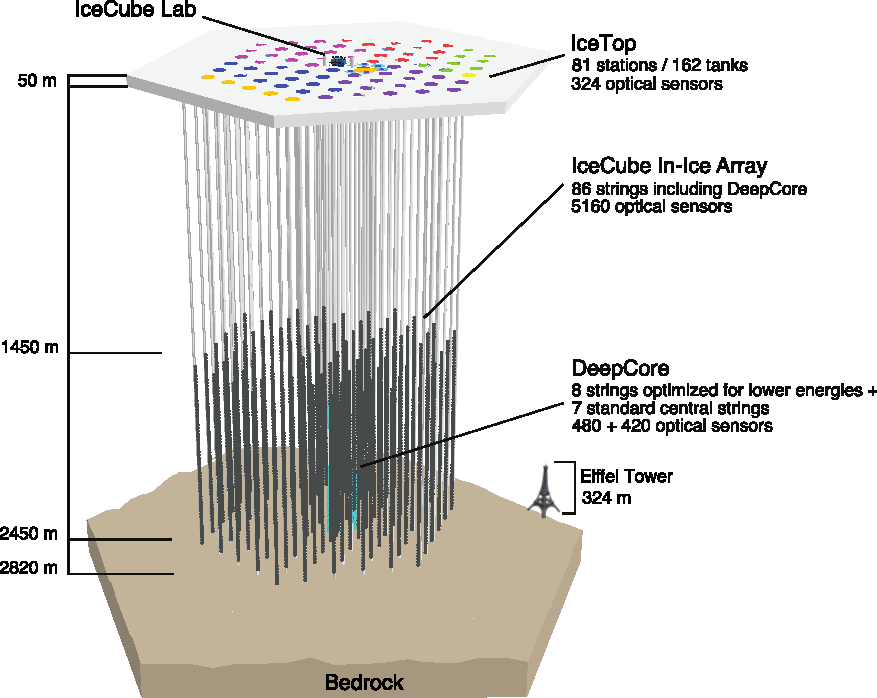
\includegraphics[width=\textwidth]{IceCubeDetector.pdf}
	\caption[Schematic view of IceCube]{\textbf{Schematic view of the IceCube Neutrino Observatory.} \cite{icecube:instrumentation} The in-ice array with the denser sub-array DeepCore as well as the surface array IceTop is sketched. Different station colors represent different deployment stages.}
	\label{icecube:detector}
\end{figure}

Neutrinos are very interesting elementary particles because of their weak interaction cross section and their electrical neutrality. This fact makes it possible for neutrinos to let them point back to their sources which is exploited in the search for astrophysical processes like active galactic nuclei, supernovae, or gamma-ray bursts. Since they are able to reach us without scattering processes, neutrinos can even give information about sources at cosmological distances. Simultaneously, the weak interaction potential is what neutrino detection makes challenging. Therefore, a detector with a large scale active volume is needed. In the case of IceCube, this is \SI{1}{\cubic\kilo\meter} of ice.

At the surface on top of the in-ice detector the cosmic ray air shower array IceTop is installed to detect Cherenkov radiation (cf. \ref{sec:cherenkov}). IceTop consists of 81 stations approximately arranged in the same grid as the in-ice strings. Each station has two tanks filled up with ice and two standard IceCube DOMs. This arrangement makes it possible for IceTop to detect primary cosmic rays (cf. \ref{sec:cosmicrays}) in the energy range of \si{\peta\electronvolt} to \si{\exa\electronvolt}. One purpose of IceTop is to provide a veto for downward-going neutrinos in the IceCube detector originating from coincident atmospheric air shower events. \cite{icecube:instrumentation} Since IceCube is investigating astrophysical neutrinos, atmospheric neutrinos are a major background.

\todo{TXS?}

\todo{IceCube-Gen2}

\section{Cosmic Rays}\label{sec:cosmicrays}

Charged particles or nuclei that are propagating through the universe and incidentally reach the Earth's atmosphere are called cosmic rays. They were discovered by the Austrian physicist \textsc{Victor Franz Hess} in 1912 when he observed an increasing discharge of electroscopes with increasing height in seven ballon flights. \cite{cosmicrays:hess} Hess initially called this underlying radiation \enquote{durchdringende Strahlung} (\textit{penetrating radiation}).

\begin{figure}[h]
	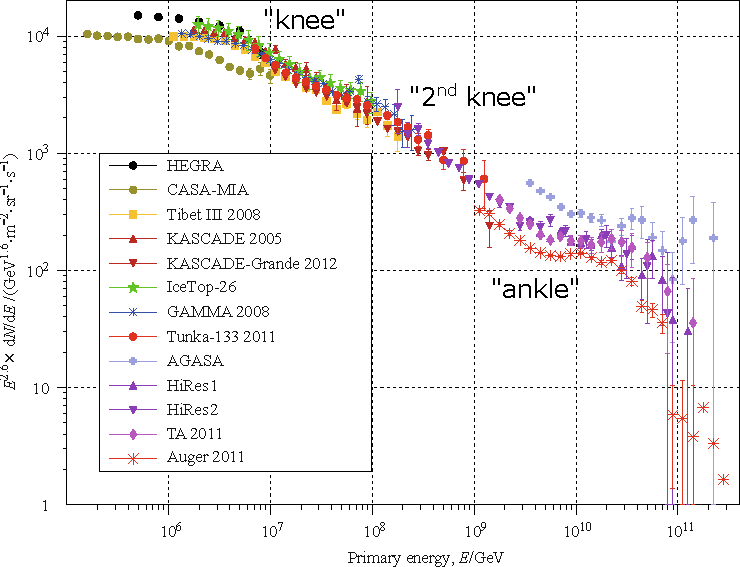
\includegraphics[width=\textwidth]{CosmicRayEnergySpectrum.pdf}
	\caption[Cosmic ray energy spectrum]{\textbf{Energy spectrum of cosmic rays measured with multiple air shower experiments.} \cite[adapted]{cosmicrays:gaisser} The three prominent regions known as \enquote{knee}, \enquote{second knee}, and \enquote{ankle} are marked. Multiplication of the spectrum by the factor $E^{2.6}$ leads to a better visibility and shows that the spectral index changes at these features.}
	\label{cosmicrays:spectrum}	
\end{figure}

When it comes to cosmic rays, ascertaining the mass composition is a key measurement for learning about their propagation in universe and about extra-galactic cosmic ray accelerators. Figure~\ref{cosmicrays:spectrum} shows that the energy spectrum of cosmic rays follows a power law:
\begin{align}
\frac{dE}{dN}\propto E^\gamma\,,
\end{align}
introducing a spectral index $\gamma$ which is dependent from the considered energy region.
Due to this interesting features, composition measurements at these \enquote{transition points} are desired in particular.

Due to the shape the spectrum is referred to as \textit{poly gonato} (Greek for \enquote{many knees}). The \enquote{knee} is assumed to be based on different rigidity\footnote{property of a magnetic field to bend a particle's trajectory} dependent cut-off energies for sub-spectra of element groups which sum up to the spectrum we observe. \cite{cosmicrays:hoerandel, cosmicrays:shapiro} At energies beyond \SI{e11}{\giga\electronvolt} a strong suppression is observed. The GZK-effect (named after Kenneth \textsc{Greisen}, Georgiy \textsc{Zatsepin}, and Vadim \textsc{Kuzmin}) is supposed to be the reason. Protons with energies above a threshold of \SI{5e19}{\electronvolt} can interact with photons of the cosmic microwave background in such a way that they produce $\pi^0$ and $\pi^+$ mesons via $\Delta^+$ resonance:
\begin{subequations}
	\begin{align}
	\gamma_\text{CMB} + p \rightarrow \Delta^+ &\rightarrow p + \pi^0\\
	&\rightarrow n + \pi^+\,.
	\end{align}
\end{subequations}
Thus, the protons effectively lose about \SI{20}{\percent} of their energy. Additionally, calculations show that these interactions become quite frequent for proton energies of $E_p\gtrsim\SI{e20}{\electronvolt}$ which results in an effective cutoff of cosmic-ray energies above this region. \cite{cosmicrays:gzk}

\section{Extensive Air Showers}

If a high energetic particle -- a photon or hadron -- incidentally reaches the Earth's atmosphere, it interacts with their atoms. A common way to describe the traversed atmospheric matter for an air shower is the \textit{slant depth}
\begin{align}
X(h) = \int_{h}^{\infty}\rho(h')dh'\,
\end{align}
with the height dependent air density $\rho(h)$. Once a high energetic \enquote{primary} particle interacts with an atmospheric atom, it initiates a cascade of secondary particles. Typically, one differentiates between hadronic and electro-magnetic cascades or showers (cf. figure \ref{airshowers:cascades}). For electro-magnetic showers or sub-showers \textit{Heitler's model} is used as a simple conception. The model is based on two-body splittings of electrons, positrons, and photons by $e^+ e^-$ pair production or bremsstrahlung which occur after a fixed distance $d=\lambda_\text{em}\ln{2}$ by using the medium-specific \textit{radiation length} $\lambda_\text{em}$. In other words: after $n$ splitting processes the shower consists out of $N = 2^n = e^{x/\lambda_\text{em}}$ electrons and photons.

\begin{figure}[h]
	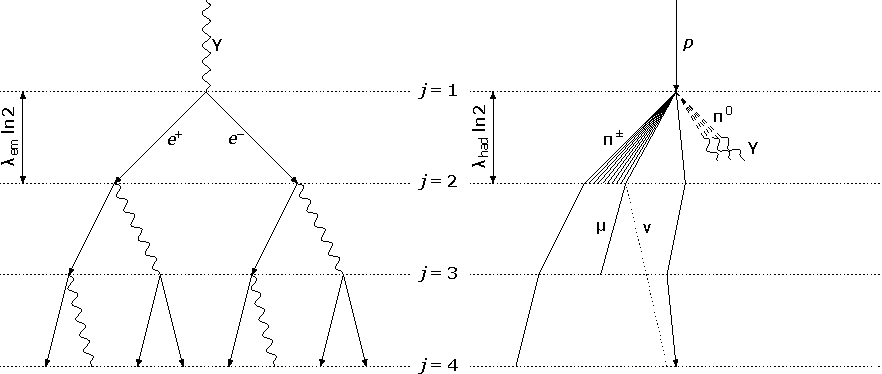
\includegraphics[width=\textwidth]{AirShowerHeitler.pdf}
	\caption[Schematic view of extensive air showers]{\textbf{Schematic view of extensive air showers.} \cite{famous:niggemann} Two possible shower formations are shown. A primary photon initiates a electro-magnetic shower (left) whereas a primary proton initiates a hadronic shower with electro-magnetic sub-showers. The splitting steps are stated as well as the interaction lengths. For the hadronic cascades not all traces are sketched for clarity reasons.}	
	\label{airshowers:cascades}
\end{figure}

The multiplication process holds, until the particle energies are high enough for pair production and bremsstrahlung. Below this energy, which Heitler named as the \textit{critical energy}~$\xi_c^e$, the shower size decreases. Hence, the maximum number of particles $N_\text{max} = 2^{n_c}$ is reached after $n_c$ splitting steps. The energy of a considered primary photon $E_\circ$ is then distributed over all secondary shower particles so that $E_\circ = \xi_c^e N_\text{max} = \xi_c^e 2^{n_c}$. With this information, one can derive the slant depth $X_\text{max}$ at which the shower has the largest size. It is
\begin{align}
	X_\text{max}^\gamma = n_c\lambda_\text{em}\ln{2} = \lambda_\text{em}\ln{\left(\frac{E_\circ}{\xi_c^e}\right)}\,.
	\label{airshowers:eq:xmax}
\end{align}
It should be mentioned that this calculation only holds for pure electro-magnetic showers which is the reason for the superscript $\gamma$ in equation \eqref{airshowers:eq:xmax}. \cite{airshowers:heitlermodel}
Since the maximum depth $X_\text{max}$ is dependent from energy and type of the primary particle it is very important for composition studies of cosmic rays. A detailed discussion on several interaction models and comparisons to simulation is done in \cite{airshowers:heitlermodel}.

\section{Detection of Air Showers via Atmospheric Cherenkov Light}\label{sec:cherenkov}

\subsection{Detection Techniques}

\begin{figure}[h]
	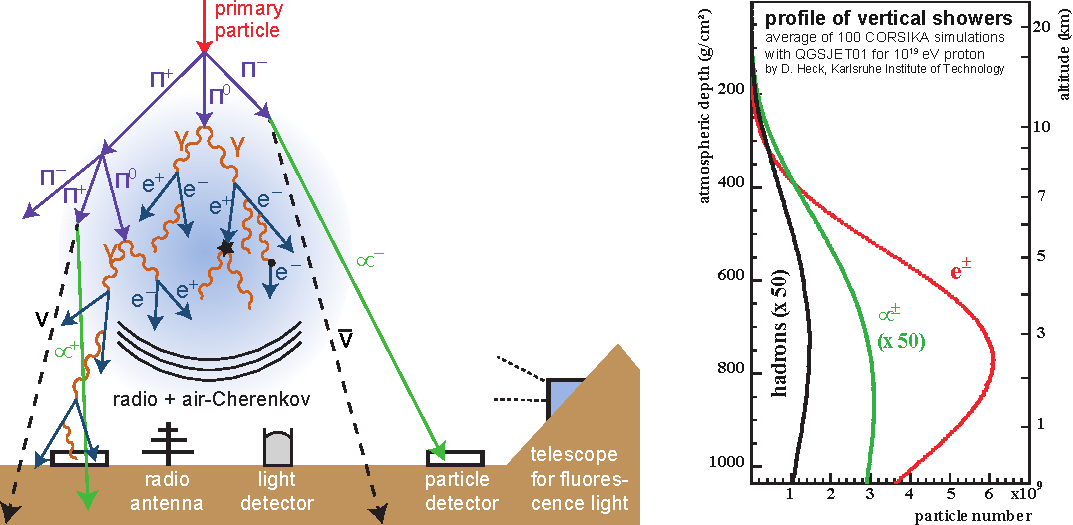
\includegraphics[width=\textwidth]{AirShowerDetection.pdf}
	\caption[Different techniques for air shower detection]{\textbf{Different techniques for the detection of atmospheric air showers.} \cite{airshowers:schroeder} }	
\end{figure}
\todo{short explanation for the different techniques}

\subsection{The Cherenkov Effect}

The Cherenkov Effect is named after the Soviet physicist \textsc(Pavel Alekseyevich Cherenkov) and describes the emission of radiation if a charged particle traverses a medium with a speed exceeding speed of light in that medium. \cite{airshowers:cherenkov} This is possible due to the fact that speed of light in a medium with a refractive index $n > 1$ is always below vacuum speed of light $c_0$ since
\begin{align}
	c = \frac{c_0}{n} \overset{n>1}{\Rightarrow} c < c_0\,.
\end{align} 
The effect is describable in two ways which are shown in figure \ref{airshowers:cherenkov}.
\begin{figure}[H]
	\centering
	\begin{subfigure}[t]{0.45\textwidth}
		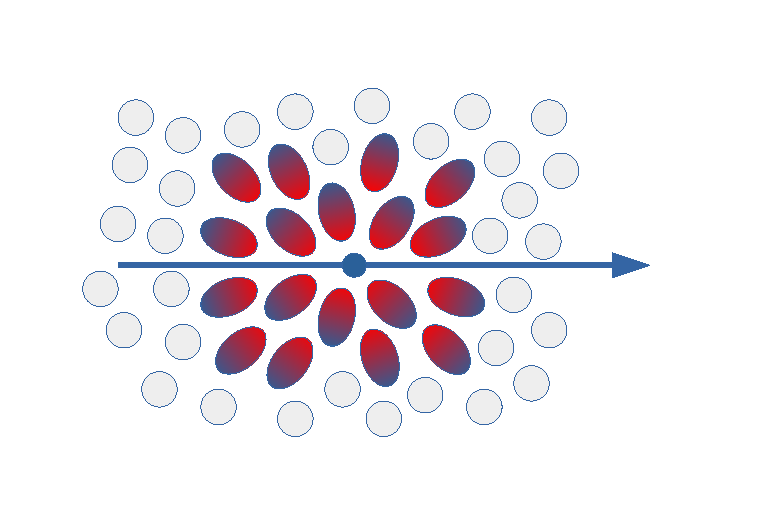
\includegraphics[width=\textwidth]{Cherenkov1Pol.pdf}
		\caption{$v < \frac{c_0}{n}$ -- The charged particle traverses the dielectric medium and polarizes its environment. For the repolarization an electric field propagates with speed of light in the medium. Since the particle's velocity is slower, no net polarization is induced and therefore no radiation is emitted.}
		\label{airshowers:cherenkov1pol}
	\end{subfigure}
	\hfill
	\begin{subfigure}[t]{0.45\textwidth}
		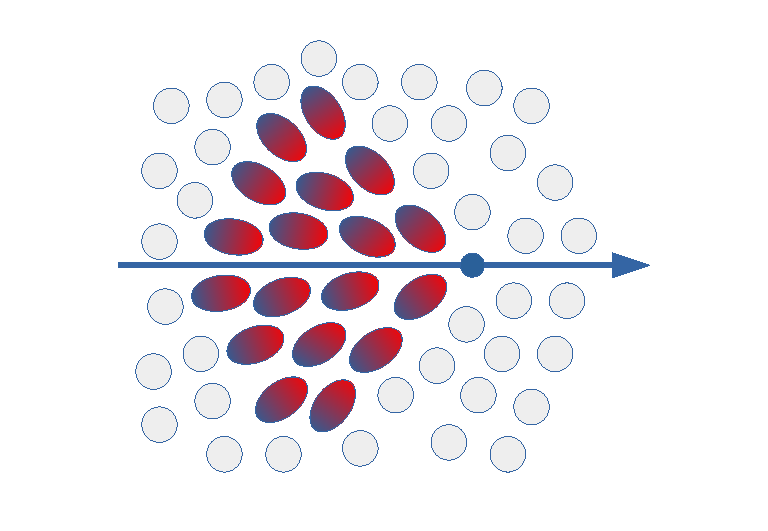
\includegraphics[width=\textwidth]{Cherenkov2Pol.pdf}
		\caption{$v > \frac{c_0}{n}$ -- The charged particles traverses the dielectric medium and polarized its environment. Since its velocity is exceeding speed of light in the medium, the electric field repolarizes the surrounding particles not fast enough so that a net polarization is induced. Cherenkov photons are emitted under a fixed angle with respect to the trajectory of the charged particle.}
		\label{airshowers:cherenkov2pol}
	\end{subfigure}
	\begin{subfigure}[t]{0.45\textwidth}
		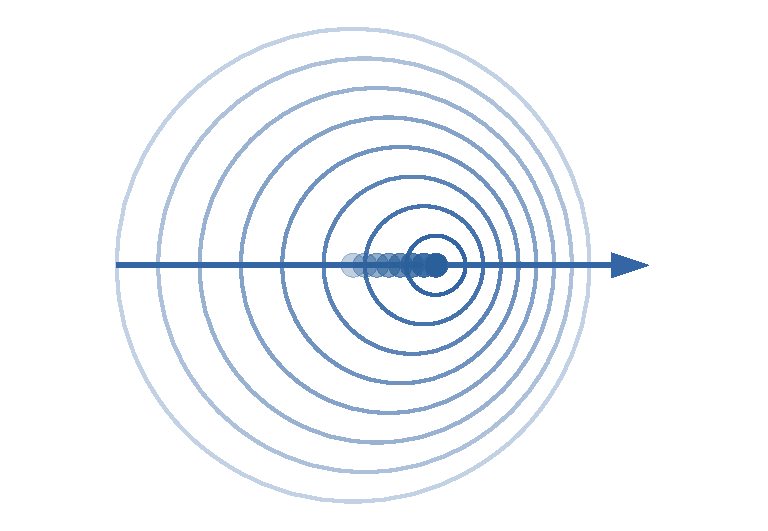
\includegraphics[width=\textwidth]{Cherenkov1Huy.pdf}
		\caption{$v < \frac{c_0}{n}$ -- The charged particle induces electro-magnetic elementary waves along its trajectory which propagate faster trough the medium than the particle. No radiation is emitted.}
		\label{airshowers:cherenkov1huy}
	\end{subfigure}
	\hfill
	\begin{subfigure}[t]{0.45\textwidth}
		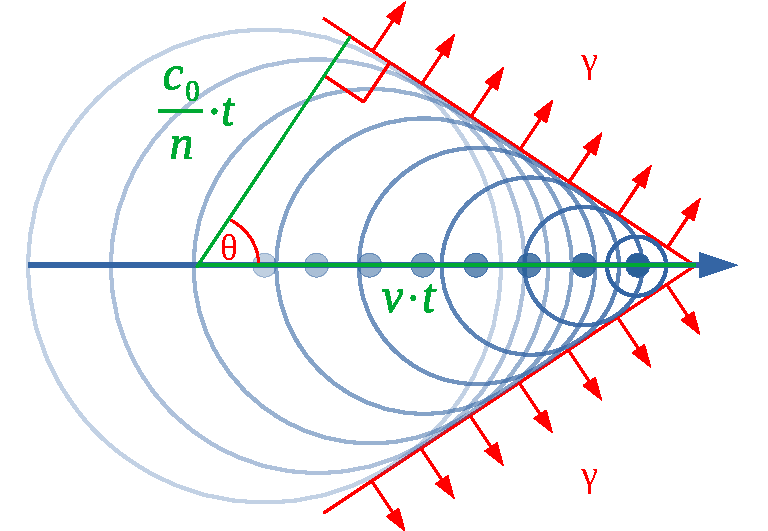
\includegraphics[width=\textwidth]{Cherenkov2Huy.pdf}
		\caption{$v > \frac{c_0}{n}$ -- The charged particle induces electro-magnetic elementary waves along its trajectory which propagate slower trough the medium than the particle. All elementary waves add up to a wavefront under a fixed angle $\theta_C$. With this model the Cherenkov effect can be interpreted as the optical analogue for the \textit{sonic boom}.}
		\label{airshowers:cherenkov2huy}
	\end{subfigure}
	\caption[Illustration for the Cherenkov effect]{\textbf{Illustration for the Cherenkov effect.} A charged particle is traversing the medium with a refractive index $n$ from left to right with velocity $v$. $c_0$ is the vacuum speed of light. In (\subref{airshowers:cherenkov1pol}) and (\subref{airshowers:cherenkov2pol}) the dipole interpretation of the Cherenkov effect is shown. (\subref{airshowers:cherenkov1huy}) and (\subref{airshowers:cherenkov2huy}) show the effect by exploiting Huygens' principle.}
	\label{airshowers:cherenkov}
\end{figure}
A \textit{Cherenkov angle} $\theta_C$ as introduced in figure \ref{airshowers:cherenkov2huy} can be calculated by applying trigonometry:
\begin{align}
	\cos{\theta_C} = \frac{c_0}{nv} = \frac{1}{n\beta}\,,
\end{align}
with the dimensionless velocity $\beta = \frac{v}{c_0}$.

Furthermore, the two Soviet physicists \textsc{Ilya M. Frank} and \textsc{Igor Y. Tamm} found a relation for the differential emission per wavelength and spatial interval known as the \textit{Frank-Tamm formula} \cite{airshowers:franktamm}:
\begin{align}
	\frac{d^2N}{dxd\lambda} = 2\pi\alpha q^2 \frac{1}{\lambda^2}\left(1-\frac{1}{n^2(\lambda)\beta^2}\right)
\end{align}
with
\begin{vardescription}
	\frac{d^2N}{dxd\lambda} & number of emitted Cherenkov photons per unit wavelength and unit propagation length\\
	\alpha & fine structure constant\\
	q & particle charge\\
	\lambda & wavelength\\
	n(\lambda) & refractive index of the medium (wavelength dependent)\\
	\beta=\frac{v}{c_0} & dimensionless relative velocity\\
\end{vardescription}
The factor $\frac{1}{\lambda^2}$ suppresses higher wavelengths so that the Cherenkov spectrum is dominant in the ultra-violet regime. Figure \ref{airshowers:cherenkovspectrum} shows a measured energy spectrum.
\begin{figure}[h]
	\centering
	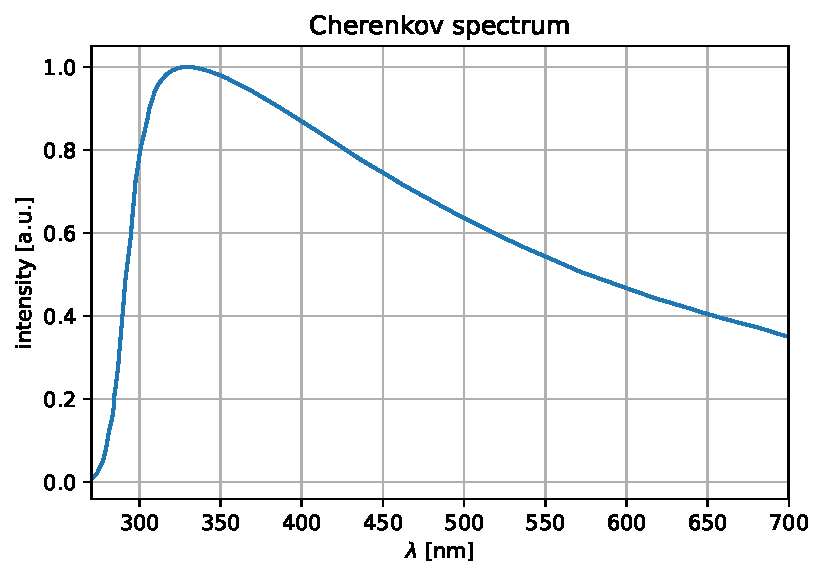
\includegraphics[width=0.5\textwidth]{CherenkovSpectrum.pdf}
	\caption[Cherenkov spectrum]{\textbf{Cherenkov wavelength spectrum.} Exemplary spectrum of Cherenkov photons measured at \SI{2200}{\meter} above sea level at the HEGRA IACT System (La Palma)\footnotemark. The falling edge towards high wavelength is proportional to $\lambda^{-2}$ whereas the falling edge towards low wavelengths is caused by atmospheric attenuation. Data adapted from \cite{airshowers:doering}.}	
	\label{airshowers:cherenkovspectrum}
\end{figure}
\footnotetext{\textbf{H}igh \textbf{E}nergy \textbf{G}amma \textbf{Ray} \textbf{A}stronomy, operated between 1987 and 2006 at Roque de los Muchachos Observatory on La Palma. \cite{airshowers:doering}}

The cone-like radiation profile of Cherenkov light with respect to the air shower axis makes it possible to reconstruct the shower direction by observing the direction of the Cherenkov photons.

\section{Imaging Air Cherenkov Telescopes}

\subsection{Imaging Technique}

\subsection{Photon Detection}

\subsection{The IceCube Air Cherenkov Telescopes IceAct}\label{sec:iceact_intro}
    % !TeX spellcheck = en_US
\chapter{The \iceact Model in \geant}

The optical system of \iceact is modeled in \geant. The following chapter will give a view on the material properties and working principles on all optical components.

\section{\geant}

\begin{wrapfigure}{r}{0.5\textwidth}
	\centering
	
\includegraphics[width=0.5\textwidth]{Geant4Logo.png}
	\caption[\geant logo]{\textbf{\geant logo.} \cite{geant4:logo}}	
\end{wrapfigure}
\geant is a multi-purpose simulation framework for the passage of particles trough matter, written in \textit{C++} and developed by the \geant Collaboration at CERN. It includes physics models, geometry, tracking, hits, and digitization. Thus, it allows detailed simulations and response analyses for particle detectors in many application fields like particle and accelerator physics, space engineering or medical science. In the framework's source some basic and advanced use cases are implemented and provided as examples. The toolkit is built up of multiple categories (or modules) using each other (cf. figure \ref{geant4:categories}).~\cite{geant4}

\begin{figure}[H]
	\centering
	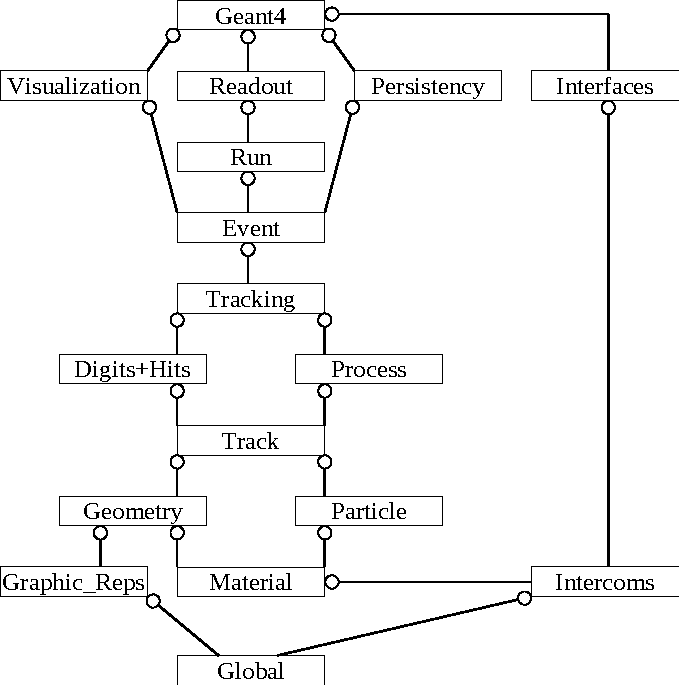
\includegraphics[width=0.5\textwidth]{Geant4ConceptDiagram.pdf}
	\caption[\geant category diagram]{\textbf{Diagram of relationships between \geant categories.} \cite[adapted]{geant4} The circles represent a \enquote{using} relation. The category with the circle next to the box uses the linked one.}	
	\label{geant4:categories}
\end{figure}

Especially for \iceact, \geant is capable of simulating Cherenkov (optical) photons, material properties like transmission, reflection, and refraction, as well as detection efficiency properties of the SiPMs.

Since this thesis is about an approach of an all-encompassing telescope simulation, \geant provides all major possibilities to get a distinct analysis of the entire optical system of \iceact.

\subsection{FAMOUS Telescope Simulation}\label{sec:famous_simulation}
The fluorescence telescope FAMOUS\footnote{\textbf{F}irst \textbf{A}uger \textbf{M}ulti-pixel
photon counter camera for the \textbf{O}bservation of \textbf{U}ltra-high-energy air \textbf{S}howers} for the Pierre Auger Observatory in Argentina is developed at RWTH Aachen to measure fluorescence light originating from ultra-high-energy cosmic rays (UHECR) by using Silicon Photomultipliers (SiPMs). Within the development, a detailed \geant simulation has been elaborated \cite{famous:sim_github,famous:sim_github}. The telescope design of FAMOUS is similar since the detection technique and the optics system is basically the same. Therefore, the \iceact telescope simulation is based on this FAMOUS \geant framework. A detailed discourse and a summary of previous analyses can be found in~\cite{famous:niggemann}.

\section{Materials}\label{sec:iceact:model:material}

For an optical device, the material that the light should pass has to be chosen deliberately. Especially the transmission properties, processability, and for \iceact in particular the resistance against harsh weather conditions are of interest.\\

The glass plate on top of \iceact is made of SCHOTT BOROFLOAT\textsuperscript{\textregistered} 33 borosilicate glass. Borosilicate is chosen for its high durability, transparency in the interesting spectral region, flatness, and weak fluorescence intensities. The refractive index is evaluated at some wavelength. Since we need to have a full dispersion relation the points are spline interpolated (cf. orange curve in figure~\ref{iceact:model:material:refractive_index}).~\cite{iceact:borosilicate:datasheet}

In the BOROFLOAT\textsuperscript{\textregistered} 33 data sheet~\cite{iceact:borosilicate:datasheet} the transmission properties are given for a vertical light and a glass plate of a thickness of $d = \SI{6.5}{\milli\meter}$. Therefore, the transmission curve $T_\text{total}(\lambda)$ includes the internal absorption as well as the two interface transitions into and out of the borosilicate which yields
\begin{align}
	T_\text{total}(\lambda) = T_\text{interface}^2(\lambda)\cdot T_\text{internal}(d=\SI{6.5}{\milli\meter},\lambda)\,.
	\label{eq:transmission}
\end{align}
The transmission at the interface can be calculated by using the Fresnel equations \cite{fresnel_equations}. In case of perpendicular light, it is
\begin{align}
	T_\text{interface}(\lambda) = 1 - \left(\frac{n(\lambda)-n_\text{air}}{n(\lambda)+n_\text{air}}\right)^2\,.
	\label{eq:perp_interface_transmission}
\end{align}
In \geant the wavelength dependent absorption length $a(\lambda)$ has to be implemented which is given by exponential absorption:
\begin{align}
	I(x) = I_0 e^{-\frac{x}{a}} \Leftrightarrow a = - \frac{x}{\ln{\frac{I(x)}{I_0}}}\,.
	\label{eq:absorptionlaw}
\end{align}
Thus, one gets the absorption length by using equations~\eqref{eq:transmission}, \eqref{eq:perp_interface_transmission}, and \eqref{eq:absorptionlaw} with
\begin{align}
	a(\lambda) &= - \frac{d}{\ln T_\text{internal}(d,\lambda)}\nonumber\\
	&= \frac{d}{2\ln\left(1 - \left(\frac{n(\lambda)-n_\text{air}}{n(\lambda)+n_\text{air}}\right)^2\right)-\ln T_\text{total}(\lambda)}\,.
\end{align}
This is implemented in the \geant material properties with $n_\text{air} = 1$. Figure \ref{iceact:model:material:transmission} shows the three transmission components as orange lines.\\

The Fresnel lens and the Winston Cones in \iceact are made of polymethyl methacrylate (PMMA). The dispersion~$n(\lambda)$ can be parametrized with the empirical \textit{Sellmeier equation}~\cite{iceact:sellmeier}. For glasses, the usual form is
\begin{align}
	n^2(\lambda) = 1 + \frac{B_1\lambda^2}{\lambda^2-C_1} + \frac{B_2\lambda^2}{\lambda^2-C_2} + \frac{B_3\lambda^2}{\lambda^2-C_3}\,,
	\label{eq:sellmeier}
\end{align}
with the \textit{Sellmeier coefficients} $B_{1,2,3}$ and $C_{1,2,3}$~\cite{iceact:sellmeier}. Table~\ref{iceact:model:pmma_sellmeiercoeffs} shows the used coefficients and the function is plotted in figure~\ref{iceact:model:material:refractive_index} (blue curve).

\begin{table}[H]
	\centering
	\begin{tabular}{c|l}
		$B_1$  & \num{0.99654}  \\
		$B_2$  & \num{0.18964}  \\
		$B_3$  & \num{0.00411}  \\
		$C_1$  & \SI{0.00787}{\micro\meter\squared}  \\
		$C_2$  & \SI{0.02191}{\micro\meter\squared}  \\
		$C_3$  & \SI{3.85727}{\micro\meter\squared}  \\
	\end{tabular}
	\caption[Sellmeier coefficients for PMMA]{\textbf{Sellmeier coefficients for PMMA.}~\cite{iceact:refractiveindex} The above-mentioned coefficients are used in the \geant material properties for PMMA. The related Sellmeier equation~\eqref{eq:sellmeier} is plotted in figure \ref{iceact:model:material:refractive_index} as the blue curve.}
	\label{iceact:model:pmma_sellmeiercoeffs}
\end{table}

For the transmission properties of PMMA, the same method as for borosilicate is used (see above). Therefore, the data stated in \cite{famous:niggemann} is taken as $T_\text{internal}(d = \SI{3}{\milli\meter})$. Figure \ref{iceact:model:material:transmission} shows the three transmission components as blue lines.

\begin{figure}[H]
	\centering
	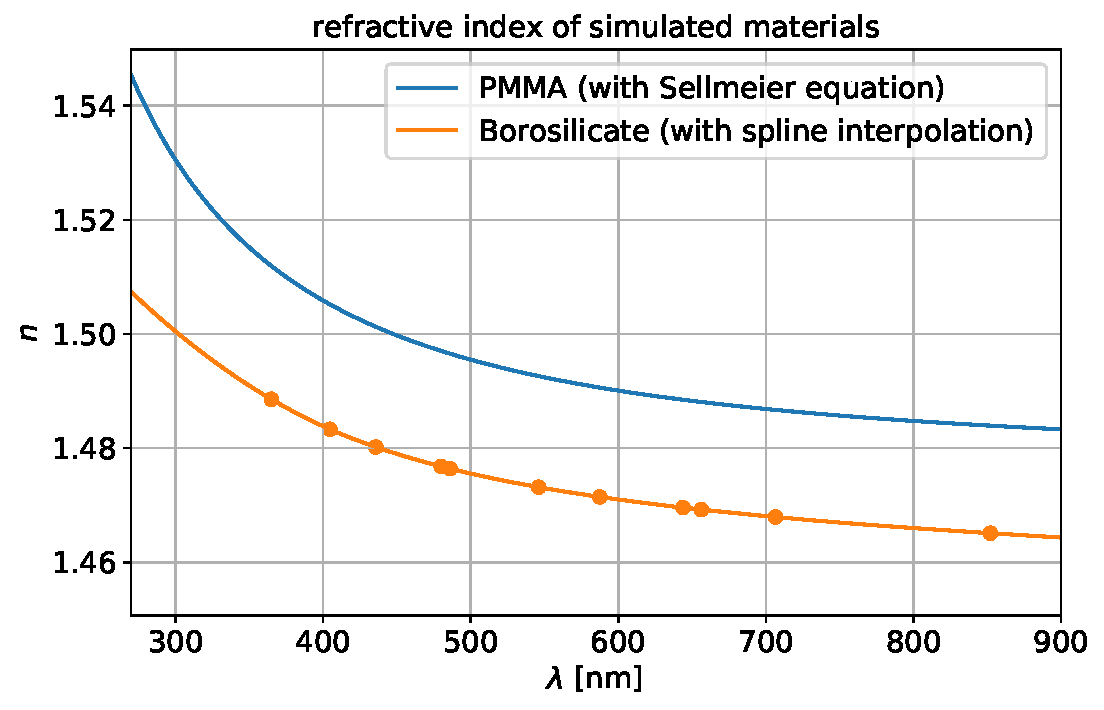
\includegraphics[width=0.7\textwidth]{material/refractive_index.pdf}
	\caption[Refractive index of used materials]{\textbf{Refractive index of materials used in the simulation.} For PMMA the dispersion is calculated by evaluating the Sellmeier equation introduced in this section. The refractive index for the used borosilicate is only given for specific wavelengths \cite{iceact:borosilicate:datasheet}. Therefore, splines are used to inter- and extrapolate the full curve.}
	\label{iceact:model:material:refractive_index}	
\end{figure}

\begin{figure}[H]
	\centering
	\begin{subfigure}[t]{0.485\textwidth}
		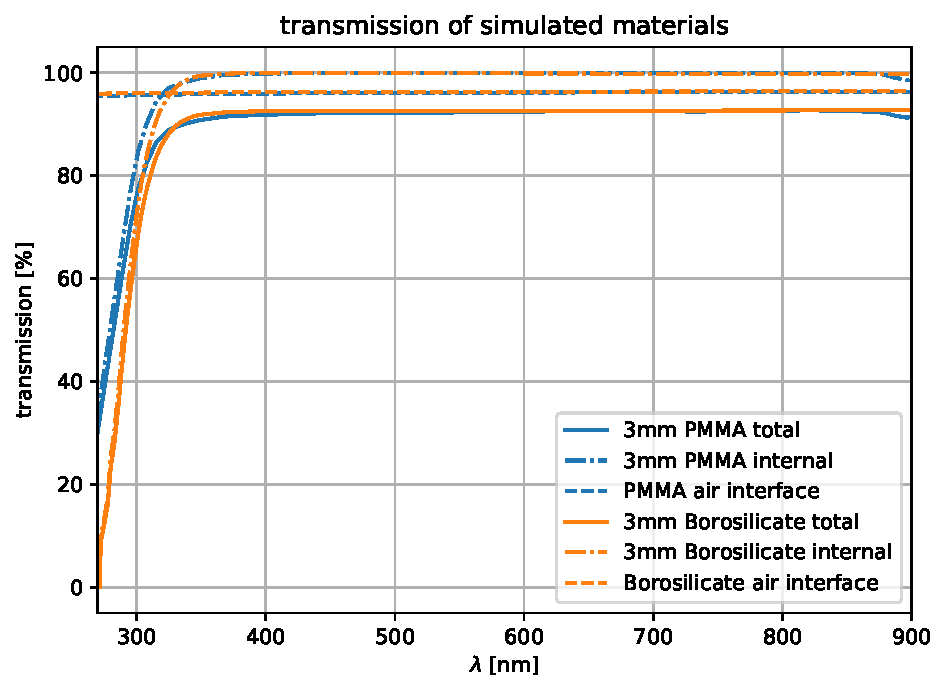
\includegraphics[width=\textwidth]{material/transmission.pdf}
		\subcaption{full view}
	\end{subfigure}
	\hfill
	\begin{subfigure}[t]{0.499\textwidth}
		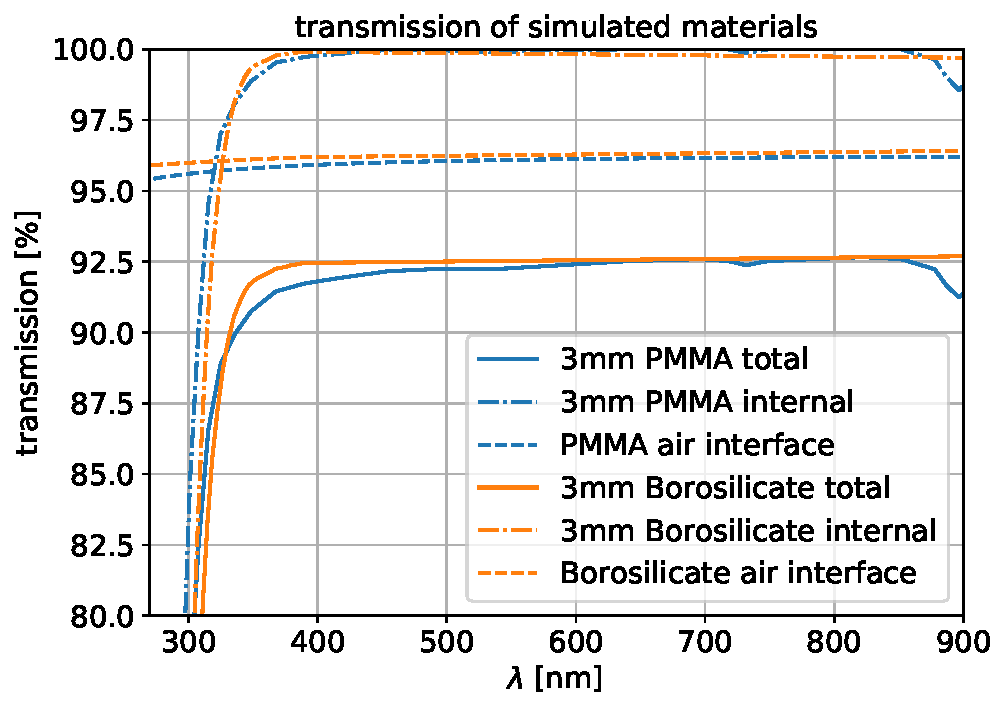
\includegraphics[width=\textwidth]{material/transmission_zoom.pdf}
		\subcaption{zoomed view}
	\end{subfigure}
	\caption[Transmission of used materials]{\textbf{Transmission functions of materials used in the simulation.} The total transmission function is the product of internal and two interface transmissions which is evaluated for a perpendicularly incident particle in this plot. Thus, the solid lines represent a complete (perpendicular) transition through a $d=\SI{3}{\milli\meter}$ thick layer of the respective material. For a better comparison, the data of internal transmission for borosilicate (given for $d=\SI{6.5}{\milli\meter}$ in~\cite{iceact:borosilicate:datasheet}) is converted for  $d=\SI{3}{\milli\meter}$.}
	\label{iceact:model:material:transmission}	
\end{figure}

The tube, back plane and other coating surfaces are simulated as \enquote{dummy} material with no reflection or transmission parameters. A particle that hits those surfaces is absorbed and not considered any further.

\section{Optics}

As introduced in section \ref{sec:iceact_intro}, \iceact is designed to image the direction of Cherenkov light on a camera consisting of multiple pixels. The imaging is done by a Fresnel lens, and an SiPM-based camera with light collecting \enquote{cones}. A sketch of the camera layout is shown in figure \ref{iceact:camera:layout}
\begin{figure}[H]
	\centering
	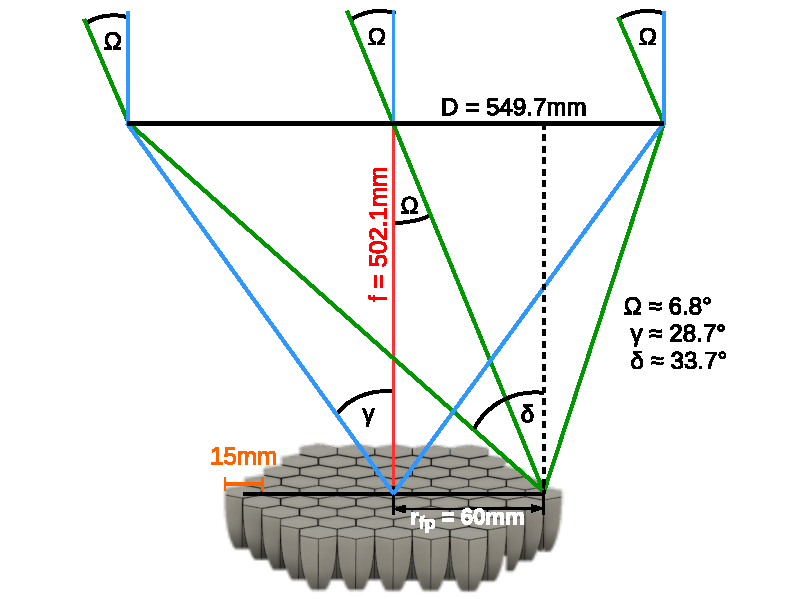
\includegraphics[width=0.6\textwidth]{CameraDesign.pdf}
	\caption[\iceact camera layout]{\textbf{The \iceact camera layout.} \cite{iceact:camera} In this sketch the Fresnel lens with a diameter $D=\SI{549.7}{\milli\meter}$ and a focal length of $f=\SI{502.1}{\milli\meter}$ focusing rays to the camera sketched below. Additionally, three characteristic angles are shown: the maximum incidence angle of a ray to be focused on the camera plane $\Omega\approx\SI{6.8}{\degree}$, the maximum incidence angle on the central Winston cone $\gamma\approx\SI{28.7}{\degree}$, and the maximum incidence angle for the outermost Winston cone $\delta\approx\SI{33.7}{\degree}$.}
	\label{iceact:camera:layout}	
\end{figure}

In the following section the four optical components of the \iceact \geant model are discussed. Figure~\ref{iceact:model:cut} shows a cross-sectional sketch of the model.
\begin{figure}[H]
	\centering
	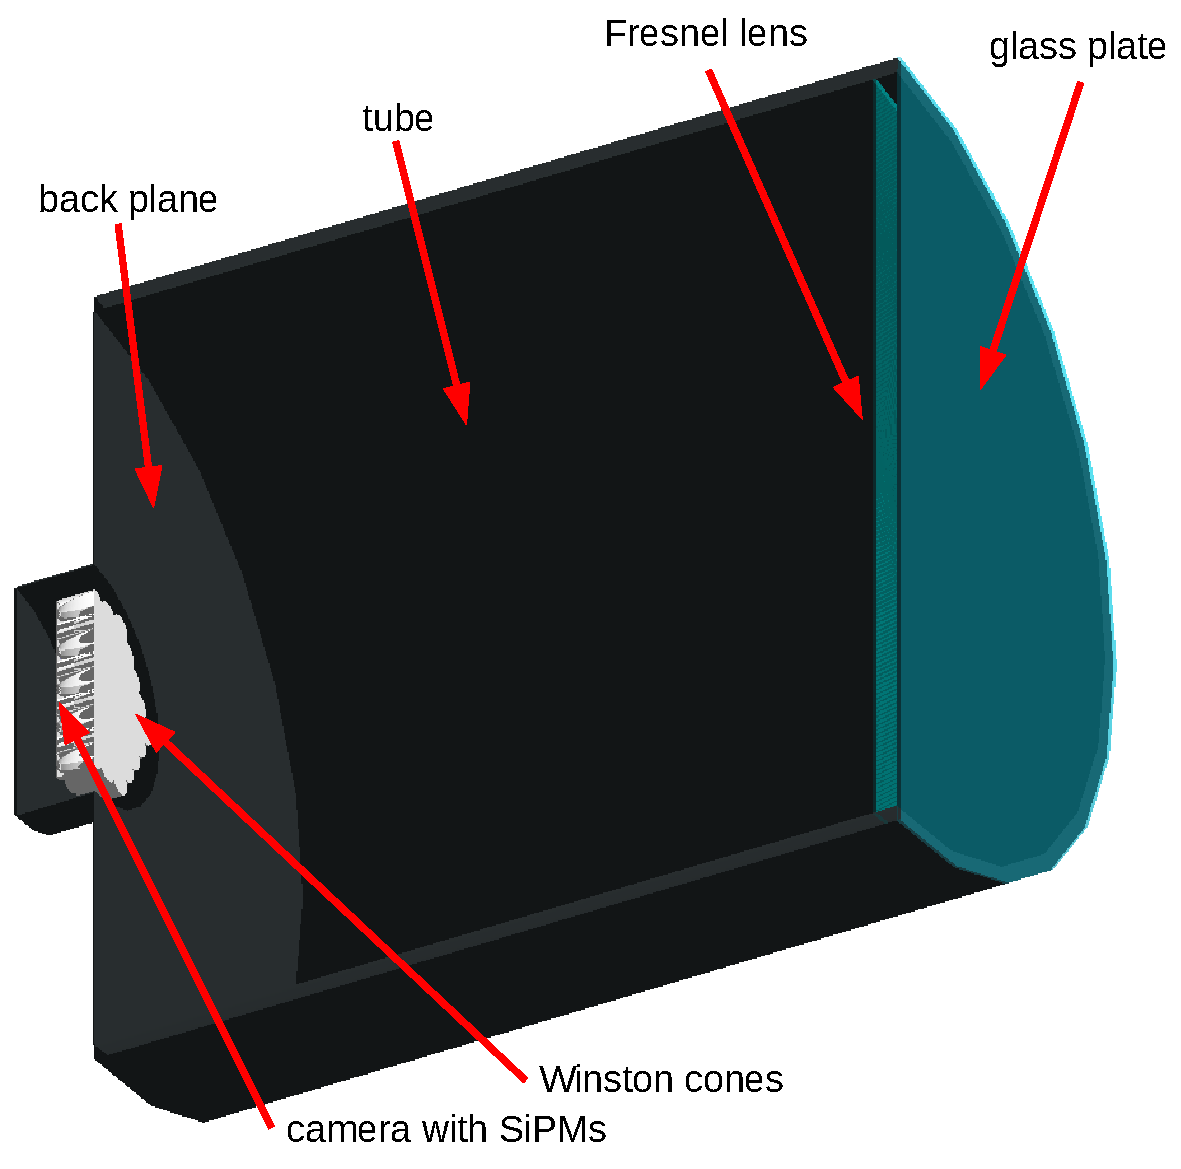
\includegraphics[width=0.6\textwidth]{IceActGeant4Model.pdf}
	\caption[\iceact \geant model]{\textbf{The \iceact \geant model.} Cross-sectional sketch of the \iceact optics in \geant with all simulated components. They are described in detail in \cref{iceact:model:fresnellens,iceact:model:camera,iceact:model:glassplate}.}
	\label{iceact:model:cut}	
\end{figure}

\subsection{Glass Plate}\label{iceact:model:glassplate}

The \iceact glass plate has a thickness of \SI{2+-0.2}{\milli\meter}, a diameter of \SI{650.3+-1}{\milli\meter}, and is made of borosilicate as mentioned in section~\ref{sec:iceact:model:material}. It is mounted on top of the tube and its major purpose is to protect the Fresnel lens from the environment. At South Pole conditions, one of the major challenges for the optical system is adherence of snow above the lens which reduces the field of view. In the \SI{12.2}{\milli\meter} thick air gap between glass plate and Fresnel lens a heating cable is installed to remove snow from the glass surface. 

\subsection{Fresnel Lens}\label{iceact:model:fresnellens}

The two major advantages using a Fresnel lens rather than a conventional lens are the significantly less weight and the fact that light passes less material which could absorb it. The main idea of a Fresnel lens is to divide a thick lens into small annular facets in form of prisms that keep the local inclination of the conventional lens by making local approximations of the lens' \textit{sagitta function}\footnote{In application to lenses, the sagitta function~$z(\rho)$ gives the lens thickness $z$ as a function of the radial distance $\rho$ from the optical axis for radially symmetrical lenses.}. Figure~\ref{iceact:model:fresnelvsthick} visualizes the principle. \iceact uses the model ORAFOL SC 943 with an aperture of \SI{549.7}{\milli\meter}, a focal length of \SI{502.1}{\milli\meter} at a wavelength of \SI{546+-27.3}{\nano\meter}. The lens is \SI{2.5}{\milli\meter} thick, has 10 grooves per \si{\milli\meter}, and is made of polymethyl methacrylate (PMMA) as stated in section~\ref{sec:iceact:model:material}.~\cite{iceact:fresnellens:datasheet}

\begin{figure}[H]
	\centering
	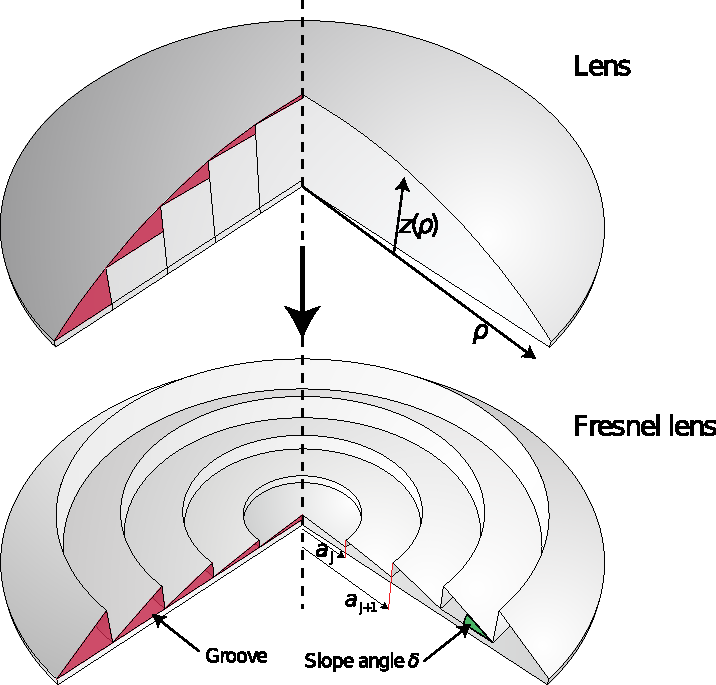
\includegraphics[width=0.5\textwidth]{FresnelVsNormalLens.pdf}
	\caption[Comparison conventional vs. Fresnel lens]{\textbf{Comparison between a conventional \enquote{thick} lens and a Fresnel lens.} \cite{famous:eichler} For the functionality of a lens the radius-dependent sagitta function $z(\rho)$ is crucial. To get rid of the bulky material of a conventional lens, the Fresnel lens is divided into annular \enquote{prisms} called \enquote{grooves}. The slope angle $\delta$ of each groove is a local approximation of the sagitta function to ensure the imaging capability.}
	\label{iceact:model:fresnelvsthick}	
\end{figure}

\begin{figure}[H]
	\centering
	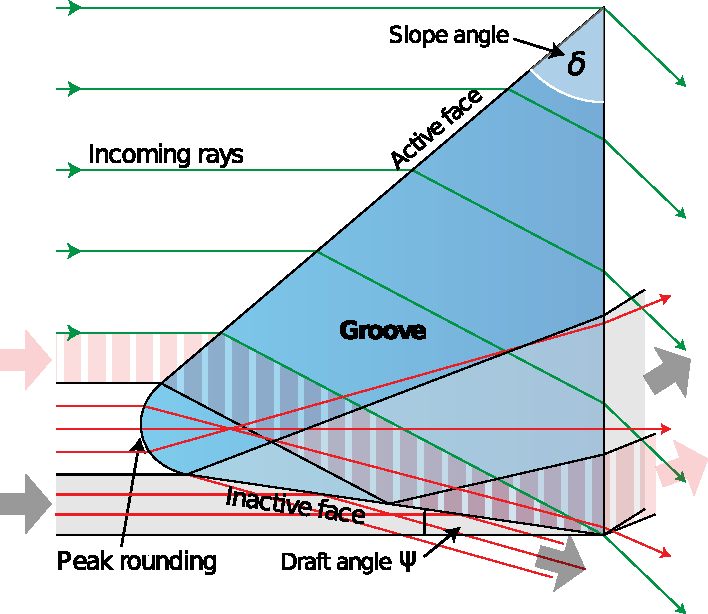
\includegraphics[width=0.5\textwidth]{FresnelGroove.pdf}
	\caption[Fresnel groove]{\textbf{Cross-sectional sketch of a Fresnel groove.} \cite{famous:eichler} Most of the incoming rays are hitting the regular active (or slope) facet of the groove with slope angle $\delta$. For an optimal groove, the inactive (or draft) facet would be parallel to the optical axis. Due to manufacturing process, there is always a small slope on the inactive facet given by the draft angle $\psi$ and the peak is rounded. With this design, there are some impact regions where incoming rays are not refracted to the focal point: if they undergo total reflection at the inactive facet inside the groove (red-dashed region), if they hit the peak rounding (red rays), or if they hit the inactive face (gray region).}
	\label{iceact:model:fresnelgroove}	
\end{figure}

\begin{figure}[H]
	\centering
	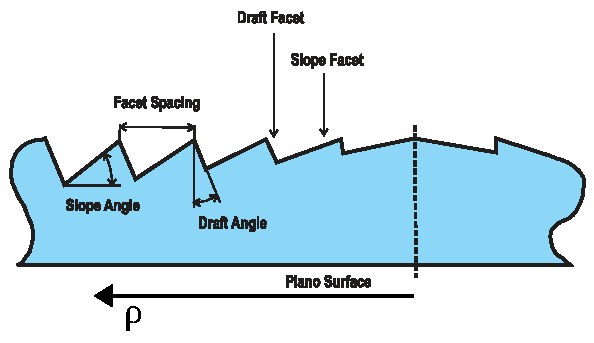
\includegraphics[width=0.5\textwidth]{FresnelSideProfile.pdf}
	\caption[Fresnel side-profile]{\textbf{Side-profile sketch of a Fresnel lens.} \cite[adapted]{iceact:fresnellens:design}. Complementary sketch to figure \ref{iceact:model:fresnelgroove} which shows the draft angle increase with radius $\rho$ driven by manufacturing.}
	\label{iceact:model:fresnelprofile}	
\end{figure}

The transmission of a Fresnel lens is not just given by the material properties. Due to the groove structure there are so called \textit{draft facets} where unwanted refractions, reflections, or transmissions occur. One can compensate for this by adjust the \text{draft angle} $\psi$ (cf. figures \ref{iceact:model:fresnelgroove} and \ref{iceact:model:fresnelprofile}) as a function of the lens radius $\rho$. Anyway, the molding process -- which is the common manufacturing technique of Fresnel lenses -- does not allow to have a perpendicular draft facet ($\psi = 0$) due to mold release. This forces the lens to have a minimum draft angle of $\psi_0 = \SI{3}{\degree}$. With the optimization mentioned before, this leads to a radial dependent draft angle which can be expressed as \cite{famous:eichler, famous:niggemann}
\begin{align}
	\psi(\rho) = \SI{3}{\degree} + \SI{0.0473}{\degree\per\milli\meter}\rho\,.
	\label{eq:draft_angle}
\end{align}\\

Nevertheless, one has to be aware of the fact that approximating a thick lens by a Fresnel lens comes along with losses due to \enquote{false} optical projections and results in aberration effects. To quantify the quality of any lens, an important property is the so called \textit{point spread function} (\textit{PSF}) which describes the energy distribution in the focal plane for a point-like light source at infinite distance, i.e. light parallel to the optical axis. One usually calculates the \textit{aberration radius} $r_{90}$. It is defined to be the radius of the circle around the PSF centroid which encloses \SI{90}{\percent} of the beam energy. One can use the aberration radius for optimizations of the optics. In more detail, this is described in section~\ref{sec:focalplaneshift}.\\

The draft angle function (cf. equation~\eqref{eq:draft_angle}) is implemented in the Fresnel lens design in \geant, the groove peak rounding suggested in figure~\ref{iceact:model:fresnelgroove} is not. The effect of simulating the rounding is discussed in \cite{famous:eichler} with the result that a peak rounding radius of $\SI{5}{\micro\meter}$ would slightly enlarge the aberration radius by a few \SI{10}{\micro\meter}. A detailed discussion and measurement of point spread functions and optical aberrations is done in \cite{famous:niggemann} and \cite{famous:eichler}.

\subsection{Camera}\label{iceact:model:camera}

\begin{figure}[H]
	\centering
	\saveimageheight[width=0.49\textwidth]{SiPMs.pdf}
	\begin{subfigure}[t]{0.49\textwidth}
		\raiseimage[width=\textwidth]{Camera.png}
		\subcaption{Picture of the assembled \iceact camera.~\cite{iceact:camera:burgmann} 61 \enquote{hex-to-square} Winston cones are glued onto the hexagonal SiPM grid. Besides, one can see two of the overall three additional pixels for reference measurements.}
		\label{iceact:camera:picture}	
	\end{subfigure}
	\hfill
	\begin{subfigure}[t]{0.49\textwidth}
		\usebox{\savedimage}
		\subcaption{Placing sketch and pixel numbering of the camera where the 61 pixels are numbered in a spiral scheme starting with the central pixel with the \geant coordinate system. In the hexagonal grid all SiPM centers have a distance of \SI{15}{\milli\meter} to their next neighboring pixels. The bright blue SiPMs are \enquote{open} pixels without a Winston cone on top and the dark blue SiPM is a \enquote{blind} pixel.}
		\label{iceact:camera:pixelnumbering}	
	\end{subfigure}
	\caption[The \iceact camera]{\textbf{The \iceact camera.}}	
\end{figure}

The \iceact camera is the compound of 61 Silicon Photomultipliers (SiPMs, cf. section~\ref{sec:sipm_working_principle}) arranged in a hexagonal grid together with 61 Winston cones (cf. section~\ref{sec:winstoncones}) glued on them. In addition to the 61 instrumented pixels there are three pixels aside for reference measurements. Two of them are just placed without Winston cones on top to measure optical noise while one pixel is completely \enquote{blind} by being masked. This makes it possible to measure the pure electronic noise of the SiPM. Figure~\ref{iceact:camera:picture} shows an assembled \iceact camera. To address each pixel, they are numbered in a spiral scheme starting with the central \enquote{0$\text{th}$} pixel and going outside counterclockwise as seen from the top (cf. figure~\ref{iceact:camera:pixelnumbering}).\\

In the following sections, the working principle as well as the implementation in \geant is discussed.

\subsubsection{Winston Cones -- Working Principle}\label{sec:winstoncones}

\begin{wrapfigure}{r}{0.5 \textwidth}
	\centering
	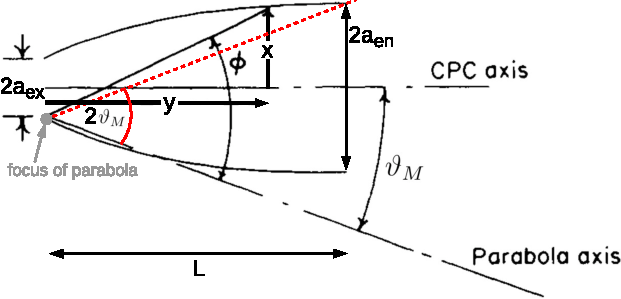
\includegraphics[width=0.5\textwidth]{WinstonConeSketch.pdf}
	\caption[Sketch of a Winston cone]{\textbf{Sketch of a Winston cone.} \cite{iceact:camera} The shape of the cone is given by the two sketched parabolic curves rotating around the CPC axis. Characteristic lengths and angles are indicated: the entrance and exit diameters $a_\text{en,ex}$, the cone length $L$, the maximum incidence angle $\vartheta_\text{M}$, the parameterization coordinates $(x,y)$, and the angle $\phi\in[\vartheta_\text{M},\vartheta_M+\SI{90}{\degree}]$ needed for parameterization as well.}
	\label{iceact:camera:wico_sketch}	
\end{wrapfigure}

The \iceact telescopes use a light collection technique to enlarge the detection area of the SiPM grid based on \textit{compound parabolic concentrators} (CPC) \cite{wico:book}. In the following, this concentrators are named \textit{Winston cones}. 
Primarily, a Winston cone is a rotationally symmetrical paraboloid formed by an off-axis parabola revolving around the axis of symmetry (\textit{CPC axis}, cf. figure \ref{iceact:camera:wico_sketch}). Hence, the entrance area $A_\text{en}=\pi a_\text{en}^2$ and the exit area $A_\text{ex}=\pi a_\text{ex}^2$ are circular. The concentration effect works for every ray hitting the entrance area up to the maximum angle $\vartheta_\text{M}$. A relation between $\vartheta_M$ and the characteristic lengths shown in figure~\ref{iceact:camera:wico_sketch} can be found: \cite{wico:book,iceact:camera}
\begin{align}
	\sin\vartheta_\text{M} = n\cdot\frac{a_\text{ex}}{a_\text{en}}\,,
	\label{eq:wico:theta_max}
\end{align}
with the refractive index $n$ of the cone material. The appearance of the refractive index connotes the to major working principles of Winston cones. On the one hand, light can be concentrated by using surface reflections in hollow cones ($n=n_\text{air}\approx 1$), or -- on the other hand -- using internal total reflections in solid cones ($n>1$). Equation~\eqref{eq:wico:theta_max} shows that the maximum angle can be increased by using a solid cone with a preferably large refractive index.

The parabola describing the Winston cone surface is further called \textit{Winston curve} and can be parameterized by \cite{wico:book,iceact:camera}
\begin{subequations}
	\label{eq:wico:param}
	\begin{align}
	x &= \frac{2a_\text{ex}(1+\sin\vartheta_\text{M})\sin(\phi-\vartheta_\text{M})}{1-\cos\phi}-a_\text{ex}\,,\\
	y &= \frac{2a_\text{ex}(1+\sin\vartheta_\text{M})\cos(\phi-\vartheta_\text{M})}{1-\cos\phi}\,,
	\end{align}
\end{subequations}

with the cone radius $x$, the cone length $y$, and the angle $\phi$ between the connecting line of focus of parabola and a point on the opposite parabola and the parabola axis (cf. figure~\ref{iceact:camera:wico_sketch}).

Another important quantity is the cone length $L$ which is given by \cite{wico:book,iceact:camera}
\begin{align}
	L = \frac{a_\text{ex}(1+\sin\vartheta_\text{M})\cos\vartheta_\text{M}}{\sin^2\vartheta_\text{M}}\sim\frac{2a_\text{en}}{2\vartheta_\text{M}}\,.
\end{align}






By appropriate design, Winston cones fulfill all requirements for light concentrators in \iceact given by the optical layout (cf. figure~\ref{iceact:camera:layout}).
However, one can design an improved Winston cone for the purposes in \iceact since a hexagonal grid of quadratic pixels with an area of $\SI{6}{\milli\meter}\times\SI{6}{\milli\meter}$ is used (cf. figure~\ref{iceact:camera:pixelnumbering}). Instead of a radially symmetrical cone, the \iceact Winston cone is designed in such a way that the exit window fits the SiPM area while the entrance window is hexagonal to maximize the camera's detectional area (cf. figure~\ref{iceact:camera:picture}). This design is called \textit{hex-to-square}. A sketch of the \iceact Winston cone is shown in figure~\ref{iceact:camera:iceact_wico_sketch}. In it, one can see a green dashed line and a pink solid line on the cone's side which follow optimized Winston curves by using the parameterization of equations~\eqref{eq:wico:param}.

\begin{figure}[H]
	\centering
	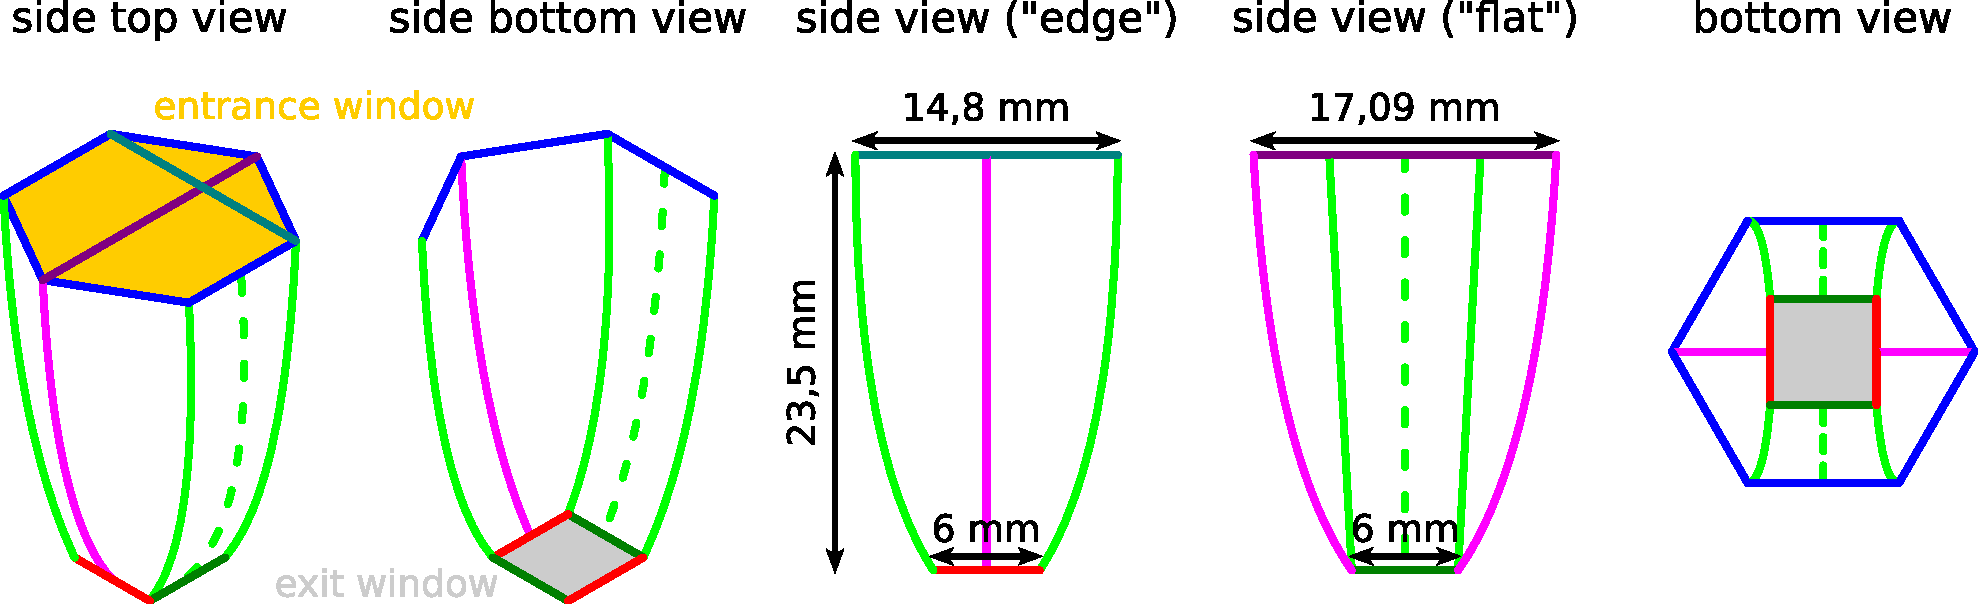
\includegraphics[width=\textwidth]{IceActWiCoSketches.pdf}
	\caption[Sketches of the \iceact \enquote{hex-to-square} Winston cone]{\textbf{Sketches of the \iceact \enquote{hex-to-square} Winston cone.} The cone is shown from different points of view with dimensioning. The pink edge and the green dashed surface line follow the optimized Winston curve functions developed in \cite{iceact:camera}. The green dashed curve is extruded in order to form the whole side. Two different functions result in two different maximum angles $\vartheta_\text{M}^\text{edge,side}$ for an incidence parallel to the \enquote{edge} or the \enquote{side} plane.}
	\label{iceact:camera:iceact_wico_sketch}	
\end{figure}

Hence, the application of Winston cones extend the detectional area of the pixels by a factor of (cf. figure \ref{iceact:camera:iceact_wico_sketch})
\begin{align}
	\frac{A_\text{camera with WiCos}}{A_\text{camera without WiCos}} = \frac{61\cdot \frac{3}{2}\sqrt{3}\cdot\left(\frac{\SI{17.09}{\milli\meter}}{2}\right)^2}{61\cdot(\SI{6}{\milli\meter})^2}\approx\num{5.27}\,.
\end{align}

\subsubsection{Winston Cone Implementation in \geant with CADMesh}

Due to its complex shape the cones are implemented in \geant by decomposing their CAD\footnote{\textbf{C}omputer-\textbf{a}ided \textbf{D}esign, technique to use a computer for the creation, analysis, etc. of a design.} sketch into small triangular tiles called \textit{meshing}. For the \iceact Winston cone this is done with the CAD software \textit{FreeCAD}, more precisely with the algorithm \textit{Mefisto}. This meshing routine only needs the maximum edge length of the single tiles as a free parameter. The smaller the maximum edge length the more detailed the mesh gets but the more computational time is needed to translate this mesh into \geant. Thus, a good compromise has to be found. Figure~\ref{wico:meshing} shows the meshed cone dependent on the maximum edge length. Simulations show a good performance for a maximum egde length of \SI{0.2}{\milli\meter}. Higher lengths result in visible image artifacts. (cf. section~\ref{sec:wico_meshing}) 

\begin{figure}[H]
	\centering
	\includegraphics[width=\textwidth]{wicomeshes/WiCo_Meshes.pdf}
	\caption[\iceact Winston cone meshing with different maximum edge lengths]{\textbf{\iceact Winston cone meshing with different maximum edge lengths.} The accuracy increases by reducing the maximum edge length of the tiles. The length of \SI{0.2}{\milli\meter} is used in the simulation.}
	\label{wico:meshing}	
\end{figure}

The meshed geometry is then translated into \geant by using the toolkit \textit{CADMesh} \cite{wico:cadmesh}. More about Winston cone meshing is discussed in section \ref{sec:wico_meshing}.

\subsubsection{Silicon Photomultipliers (SiPM)}\label{sec:sipm:working_principle}

Silicon Photomultipliers (\textit{SiPM}s) are semiconductor devices used for photon detection in multiple applications. In comparison to conventional photon detection devices like Photomultiplier Tubes (\textit{PMT}s) they are rather compact and offer a higher detection efficiency. These features made them interesting devices for application in imaging detectors.

An SiPM is the composition of an array of so called \textit{Geiger-mode avalanche photo diodes} (\mbox{\textit{G-APD}s}). Their working principle is based on $p$-$n$-junctions (cf. figure~\ref{sipm:pn_junction}). This is the simple configuration when an $n$-doped and a $p$-doped material are brought together. Thus, a \textit{depletion zone} occurs where free electrons of the $n$-doped material fill holes of the $p$-doped material. Due to the resulting net charge, an electric field arises from the $n$- to the $p$-doped side, comparable to a capacitor. The size of the depletion zone can be enlarged by an external \textit{bias voltage} $V_\text{bias}$ applied with the anode side at the $n$-doped material. In this state, the junction conducts current easily only in one direction, which is commonly known as a \textit{diode}. \cite{pn:simon}

\begin{figure}[H]
	\centering
	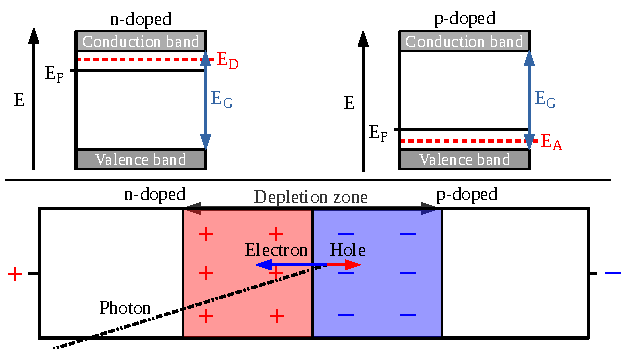
\includegraphics[width=0.7\textwidth]{PNJunction.pdf}
	\caption[Sketch of a $p$-$n$-junction]{\textbf{Sketch of a $p$-$n$-junction.} \cite{iceact:camera} In the top, the energy bands are shown for $n$-doped and $p$-doped semiconductor with the Fermi energy level $E_F$, the gap energy $E_G$, and the donor or acceptor energy level $E_D$ and $E_A$ respectively. Below, a $p$-$n$-junction is sketched. An incident photon may result in production of an additional electron-hole-pair inducing a current via avalanches.}
	\label{sipm:pn_junction}	
\end{figure}

If a photon now traverses the diode, a possible impact can ionize an atom and thus produce an electron-hole-pair. While the electron is accelerated along the electrical field it can ionize further atoms if the electric field is strong enough -- an avalanche is formed that induces a highly temperature-dependent breakdown voltage $V_\text{breakdown}$. Here, the \enquote{Geiger-mode} prefix additionally indicates that the signal is not dependent on the number of total detected photons. A quenching resistor allows to stop the avalanche and enables the cell to recover quickly. This working principle is referred to as an \textit{avalanche photo diode} (\textit{APD}). Usually, photo diodes are based on germanium (Ge) or silicon (Si). Since the band gap of silicon-based photo diodes is higher (\SI{1.12}{\electronvolt}) than for germanium-based ones (\SI{0.67}{\electronvolt}), the electrons in silicon-based photo diodes need higher energies to produce a significant photo currents. Thus, Si photo diodes generate less noise than photo diodes based on Ge. \cite{sipm:renker_lorenz} An important operation parameter of a G-APD is the over voltage $V_\text{OV}$ since many features (e.g. the gain) of G-APDs are proportional to it. It is defined as the difference of bias and breakdown voltage~\cite{sipm:renker_lorenz}
\begin{align}
	V_\text{OV} = V_\text{bias} - V_\text{breakdown}\,.
\end{align}

Basically, there are two types of G-APD cells: $p$-on-$n$ which is shown in figure~\ref{sipm:apd_cell} and $n$-on-$p$. They differ in the wavelength region they are efficient in. While $n$-on-$p$ cells are efficient for wavelengths beyond \SI{1}{\micro\meter}, the $p$-on-$n$ cells operate best in the blue and UV regime -- thus in the peak region of Cherenkov light (cf. figure~\ref{airshowers:cherenkovspectrum}).

\begin{figure}[H]
	\centering
	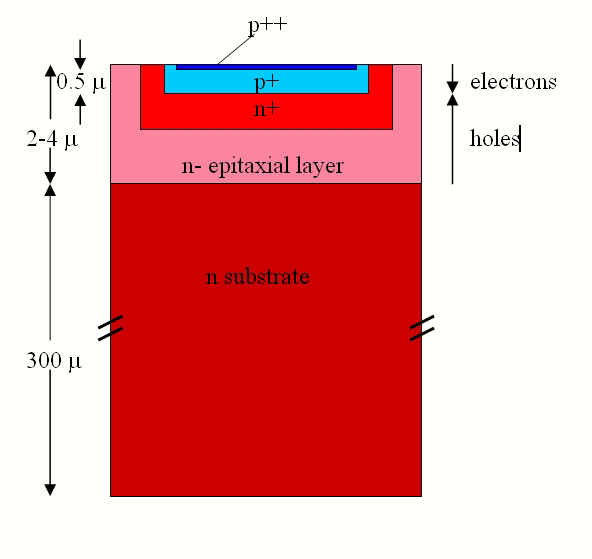
\includegraphics[width=0.5\textwidth]{APD_Cell.png}
	\caption[Sketch of a \enquote{$p$-on-$n$} G-APD cell]{\textbf{Sketch of a \enquote{$p$-on-$n$} G-APD cell.} \cite{sipm:renker_lorenz} This type is optimized to have a high photon detection efficiency in the blue and UV wavelength regime.}
	\label{sipm:apd_cell}	
\end{figure}

\begin{figure}[H]
	\centering
	\saveimageheight[width=0.34\textwidth]{SiPM_circuit.pdf}
	\begin{subfigure}[t]{0.62\textwidth}
		\raiseimage[width=\textwidth]{SiPM_picture.png}
		\subcaption{Picture of the MicroFJ-60035-TSV SiPM which is used in the \iceact camera as seen from the top (left) and the back (right). One can slightly see the fine grid of \num{22292} G-APDs with a size of $\SI{35}{\micro\meter}\times\SI{35}{\micro\meter}$ arranged on a package with the dimensions $\SI{6.07}{\milli\meter}\times\SI{6.07}{\milli\meter}$.}
		\label{sipm:iceact_sipm}
	\end{subfigure}
	\hfill
	\begin{subfigure}[t]{0.34\textwidth}
		\usebox{\savedimage}
		\subcaption{Circuit diagram of a SiPM with 12 (very few) G-APD cells in parallel connection. One can see that each cell has its own quenching resistor. The fast output is not used in the application for \iceact.}
	\end{subfigure}
	\caption[Structure of an SiPM]{\textbf{Structure of an SiPM.} \cite{sipm:datasheet}}
	\label{sipm:circuit_picture}
\end{figure}

The step from a G-APD to an SiPM is done if one now combines many G-APDs in a grid structure in parallel connection which is shown in figure~\ref{sipm:circuit_picture}. Figure~\ref{sipm:pulses} shows measured waveforms (or \enquote{pulses}) of SiPM with linear amplification. A discretization of puls heights which correspond to the number of single cell breakdowns can be observed. The amplitude $A_i$ of a standard pulse is proportional the capacitance $C$ and anti-proportional to the electron charge $q$ and the over voltage $V_\text{OV}$,~\cite{sipm:renker_lorenz}
\begin{align}
	A_i\propto\frac{C}{qV_\text{OV}}\,.
\end{align}
If now multiple cell breakdowns occur, the total pulse height just sums up over the number of triggered cells which is commonly knows as \textit{PE} (\textit{photo electron equivalent}),~\cite{sipm:renker_lorenz}
\begin{align} 
	A = \sum_{i=0}^{PE} A_i\,.
\end{align}

\begin{figure}[H]
	\centering
	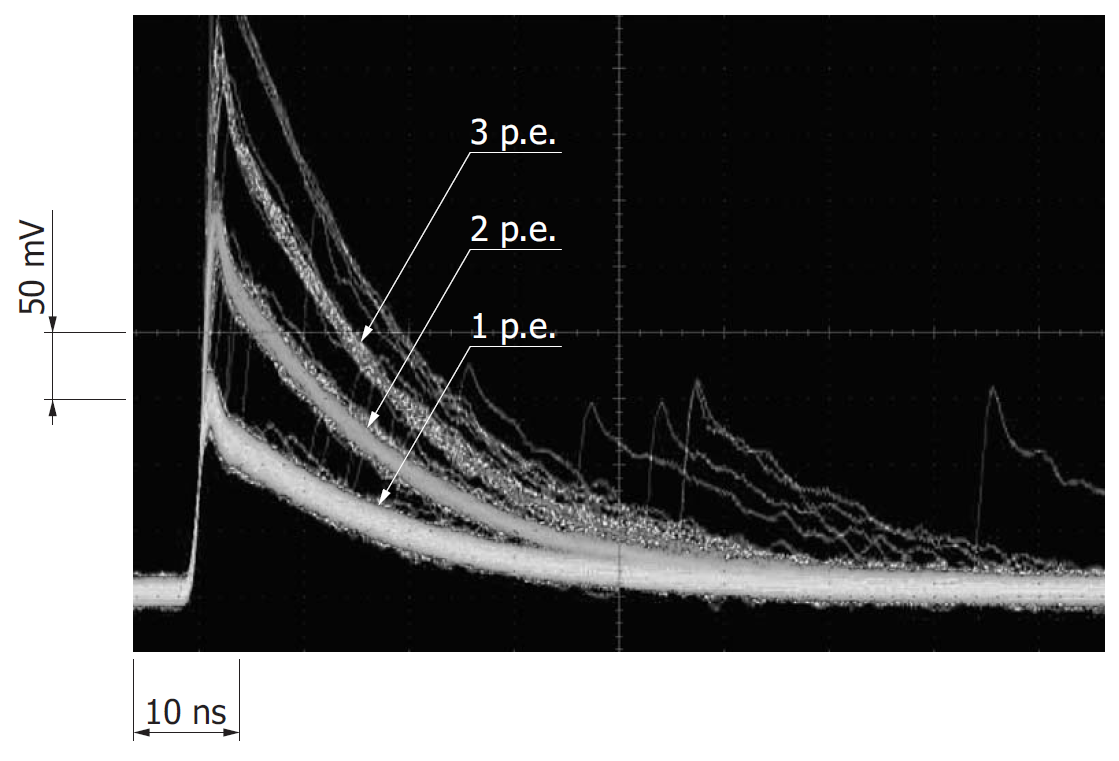
\includegraphics[width=0.7\textwidth]{SiPM_pulseplot}
	\caption[Pulse waveforms of an SiPM]{\textbf{Pulse waveforms of an SiPM.} \cite{sipm:hamamatsu_handbook} Multiple measured SiPM waveforms (\enquote{pulses}) with amplitude plotted against time. A discretization of pulse heights can be observed which is dependent on the number of single cell breakdowns marked with \enquote{p.e.} in the plot. One can see a few after pulses at later times as well.}
	\label{sipm:pulses}
\end{figure}

In addition, the pulse shape can be parameterized by a function of two exponential functions,
\begin{align}
	A(t,PE) = c\cdot PE \cdot \left(1-\frac{1}{1+\exp\left(\frac{t-t_0}{\tau}\right)}\right)\cdot\exp\left(-\frac{t-t_0}{\lambda}\right)\,,
\end{align}
where $c$ is a calibration factor, that corresponds to the amplitude of a \SI{1}{PE} pulse, $t_0$ is the starting time of the pulse, and $\tau$ and $\lambda$ are the rise and fall times respectively, which are typically in a range of $\tau=\SI{0.9}{\nano\meter}$ to $\SI{1.1}{\nano\meter}$ and $\lambda=\SI{18}{\nano\second}$ to $\SI{20}{\nano\second}$.~\cite{sipm:fact_calibration}

Moreover, figure~\ref{sipm:iceact_sipm} shows the SiPM used for the \iceact camera. It is the MicroFJ-60035-TSV SiPM by ON Semiconductor\footnote{In former theses and publications on \iceact the SiPM is called SensL J-Series 60035. Since 2018, SensL is fully integrated in the head organization ON Semiconductor which took over the sales of SensL products.}. 
It consists of \num{22292} G-APD cells with the dimensions $\SI{35}{\micro\meter}\times\SI{35}{\micro\meter}$ each. The active area is $\SI{6.07}{\milli\meter}\times\SI{6.07}{\milli\meter}$ and the package area is $\SI{6.13}{\milli\meter}\times\SI{6.13}{\milli\meter}$ which results in a fill factor\footnote{Percentage of the active area that is actually equipped with cells.} of $\epsilon_\text{fill}=\SI{75}{\percent}$. On top of the active area, a glass plate with a thickness of \SI{0.37}{\milli\meter} (cf. figure~\ref{sipm:tec_sketch}). More technical properties can be found in the data sheet~\cite{sipm:datasheet}.

\begin{figure}[H]
	\centering
	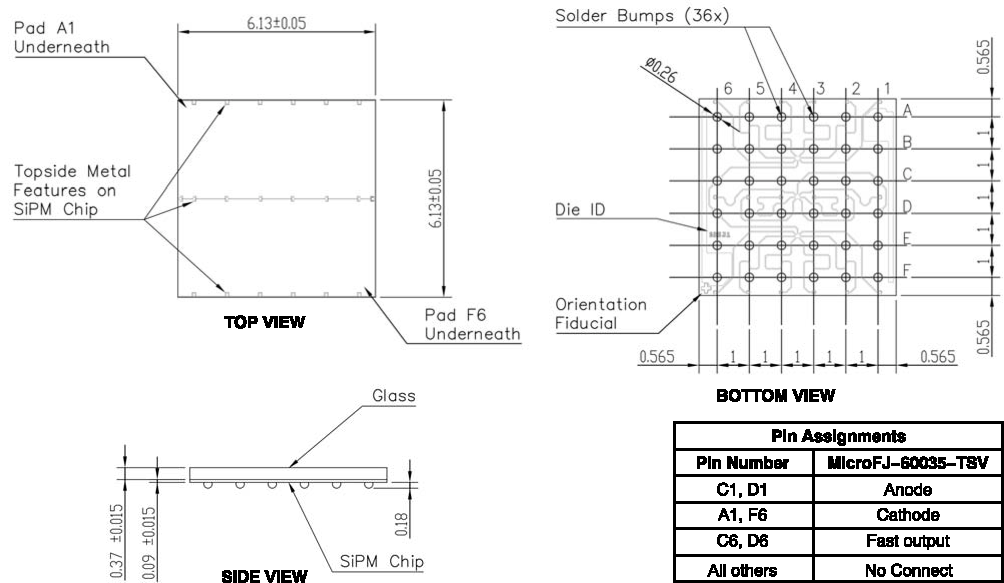
\includegraphics[width=\textwidth]{SiPM_sketch.pdf}
	\caption[Technical sketch of the MicroFJ-60035-TSV SiPM used in \iceact]{\textbf{Technical sketch of the MicroFJ-60035-TSV SiPM used in \iceact.}~\cite{sipm:datasheet} All dimensions given in \si{\milli\meter}.}
	\label{sipm:tec_sketch}	
\end{figure}

\subsubsection{SiPM Implementation in \geant with G4SiPM}

In the \iceact \geant simulation, the SiPM is implemented via the plug-in \textit{G4SiPM}~\cite{sipm:g4sipm}. It allows a convenient implementation of geometry, materials, photon detection efficiency, and many other physics and performance parameters in \geant. It is even possible to do waveform simulation with background from cross talk, after pulses, thermal noise, etc. Since the signal simulation is beyond the scope of this thesis, only the material and detection properties are of interest.\\

For the material properties of the \SI{0.37}{\milli\meter} thick covering glass plate on the SiPM, only the refractive index of $n = \SI{1.53}{\nano\meter}$ at a wavelength of $\lambda = \SI{436}{\nano\meter}$ is given in the data sheet~\cite{sipm:datasheet}. Since there are no detailed information about the glass, $n$ is assumed to be constant for the simulation.\\

The other important property is the \textit{photon detection efficiency} $PDE(\lambda,V_\text{OV})$ which is given for the over voltages $V_\text{OV}=\SI{2.5}{\volt}$ and $V_\text{OV}=\SI{6}{\volt}$ and for wavelengths $\lambda = \SI{200}{\nano\meter}$ to $\SI{900}{\nano\meter}$. In \iceact the SiPMs are operated with an over voltage of $V_\text{OV} = \SI{5}{\volt}$. Measurements in the data sheet show that the relation between over voltage and PDE is linear.~\cite{sipm:datasheet} Therefore, one gets the needed $PDE_{\SI{5}{\volt}}\coloneqq PDE(\lambda,V_\text{OV}=\SI{5}{\volt})$ by linear interpolation,
\begin{align}
	PDE_{\SI{5}{\volt}} = PDE_{\SI{2.5}{\volt}} + \frac{\SI{2.5}{\volt}}{(6-2.5)\si{\volt}} \cdot (PDE_{\SI{6}{\volt}}-PDE_{\SI{2.5}{\volt}}),
\end{align}
which is then implemented in \geant. In addition, G4SiPM takes into account, that the PDE is measured for perpendicular light incidence in air environment. By using Fresnel equations it compensates for slant photon incidences. The fill factor $\epsilon_\text{fill}$ is also divided out. \cite{sipm:g4sipm,famous:niggemann}. 
The interpolated and original PDE functions are shown in figure~\ref{sipm:pde}

\begin{figure}[H]
	\centering
	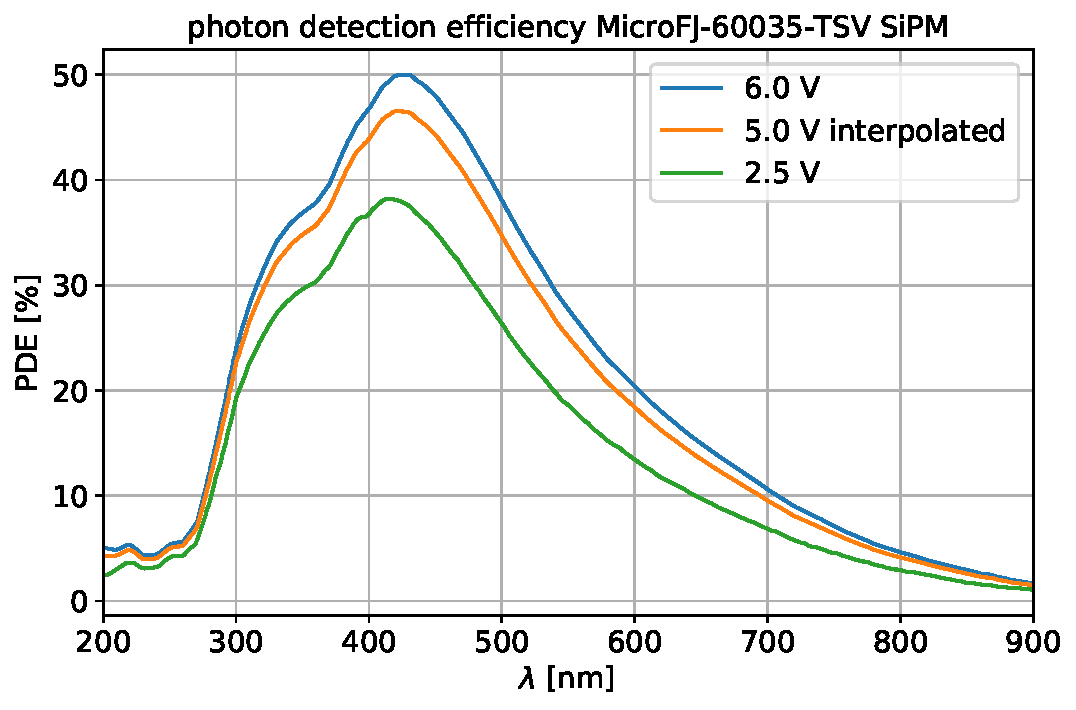
\includegraphics[width=0.7\textwidth]{material/PDE_interpolation.pdf}
	\caption[Photon detection efficiency of the MicroFJ-60035-TSV SiPM]{\textbf{Photon detection efficiency of the MicroFJ-60035-TSV SiPM.} The data for over voltages of \SI{6}{\volt} and \SI{2.5}{\volt} is taken from~\cite{sipm:datasheet}, the curve for \SI{5}{\volt} -- which is used in the \geant simulation -- is interpolated linearly.}
	\label{sipm:pde}	
\end{figure}

    % !TeX spellcheck = en_US
\chapter{Simulation Results}\label{chap:simresults}

In this chapter

\section{Simulation Strategy and Verification}

\subsection{Winston Cone Meshing}\label{sec:wico_meshing}

\subsection{Aberration Effects -- \enquote{Ghost Image}}

\section{Simulation of Single Components}

\subsection{\enquote{Best} Wavelength}

\subsection{Focal Plane Shift}
    % !TeX spellcheck = en_US
\chapter{\iceact Parameterization}

The simulation results discussed in chapter \ref{chap:iceact_sim} can now be used to parameterize the telescope response of \iceact. The major goal of this is to provide a fast way to evaluate the detection probability of incident photons in each camera pixel which is done by elaboration of a lookup table (\textit{LUT}). Afterwards, the high computational effort by propagating each Cherenkov photon through the whole \geant model is not needed any more. To achieve this, one needs a well-defined strategy to convert the simulated raw data into a meaningful parameterization. 

\section{Parameterization Strategy}\label{sec:param:strategy}

The following sections discuss the step-by-step strategy to get \textit{detection efficiency maps} out of the \geant data. These maps will describe the direction-dependent detection probabilty for a certain wavelength range and a certain camera pixel.

\subsection{Kernel Density Estimation (KDE)}

\textit{Kernel density estimation} (\textit{KDE}) is a non-parametric\footnote{A non-parametric method names a statistical approach based on a non-defined model that is deduced directly from data.} method to estimate a probability density function of a random variable by a given finite data sample. The standard \textit{kernel density estimator}
\begin{align}
	\hat{f}(x)=\frac{1}{nh}\sum_{i=1}^{n}K\left(\frac{x-X_i}{h}\right)\,,
	\label{eq:kde}
\end{align}
is the sum of \textit{kernel functions} $K(\dots)$ for each data point $X_i$. The non-negative parameter $h$ is the \textit{bandwidth} and is a measure for the smoothing of the resulting KDE: the KDE gets smoother with increasing $h$. Due to the normalization factor, $\hat{f}(x)$ is normed to
\begin{align}
	\int\limits_{-\infty}^{+\infty}\hat{f}(x)dx \equiv 1\,.
	\label{kde:norm}
\end{align}

\begin{figure}[H]
	\centering
	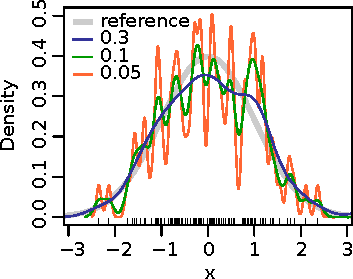
\includegraphics[width=0.5\textwidth]{KDE_example.pdf}
	\caption[Example KDE with different smoothing]{\textbf{Example KDE with different smoothing.} \cite{kde:example_plot} Kernel density estimation is applied on a data sample with 100 random numbers drawn from a normal distribution (gray curve). The blue, green, and orange curves have different bandwidths.}
	\label{kde:example_1d}	
\end{figure}

The kernel function can be a very distinct function that can in principle describe any probability density. In this parameterization method a Gaussian kernel
\begin{align}
	K(t) = \frac{1}{\sqrt{2\pi}}e^{-\frac{1}{2}t^2}
\end{align}
is used.

In order to get the KDE describing the probability density appropriately, one has to choose a reasonable bandwith for the given data sample size. As shown in figure \ref{kde:example_1d}, too low bandwith results in a spiky, fluctuating KDE. If the bandwidth is too high, one might get a rather inaccurate estimator. Therefore it seems reasonable to choose different bandwidth in regions with different amount of statistics which then is called \textit{adaptive} kernel density estimation. \cite{kde:schoenen, kde:wangwang}

\subsubsection{Adaptive KDE with Gaussian Kernel}\label{sec:adaptive_kde}

On the \iceact camera, each pixel has a certain region of photon directions where it is efficient. However, each pixel is almost \enquote{blind} for most other directions. This results in statistically stable -- \enquote{dense} -- regions but also \enquote{sparse} regions dominated by scattered photons that undergo large statistical fluctuations. Thus, and based on the former conclusions, an approach to adapt the bandwidth to the local statistics should perform well. In this thesis, an algorithm presented by \textsc{B. Wang} and \textsc{X. Wang} in \cite{kde:wangwang} which has been implemented within the scope of \cite{kde:schoenen} is used. The adaptive (in principle weighted) kernel density estimator is calculated by \cite{kde:schoenen,kde:wangwang}
\begin{align}
	f(\vec{x}) = \sum_{i=1}^{n} \frac{w_i}{N_i}e^{-\frac{1}{2}(\vec{x}-\vec{X_i})^T \frac{1}{h\lambda_i} \mathbf{C}^{-1} (\vec{x}-\vec{X_i})}\,,
\end{align}
with
\begin{vardescription}
	n & total number of data points,\\
	w_i & weight of th $i$-th data point,\\
	N_i & Gaussian normalization,\\
	\vec{X_i} & coordinate vector of the $i$-the data point,\\
	h & global bandwidth factor,\\
	\lambda_i & local bandwidth factor,\\
	\mathbf{C} & covariance matrix.\\
\end{vardescription}
The global bandwidth factor $h$ is calculated by the \textit{Silverman rule} \cite{kde:schoenen,kde:wangwang}
\begin{align}
	h = \left(\frac{n(d+2)}{4}\right)^{-\frac{1}{d+4}}\,,
\end{align}
where $d$ equals the number of dimensions of the data (here $d=2$). The local bandwidth $\lambda_i$ is the factor where the local statistics of each data point comes in. It is defined as \cite{kde:schoenen,kde:wangwang}
\begin{align}
	\lambda_i = \left(\frac{\hat{f}(\vec{X_i})}{g}\right)^{-\alpha}\,,
\end{align}
with
\begin{vardescription}
	\hat{f}(\vec{X_i}) = f(\vec{X_i})|_{w_i=\lambda_i=1}\,,\\
	\ln{g} = n^{-1} \sum_{i=1}^{n} \ln{\hat{f}(\vec{X_i})}\,,\\
	\alpha\in[0,1]\,.
\end{vardescription}
For the \iceact parameterization the sensitivity parameter $\alpha$ is set to $\alpha=\num{0.3}$, since this has been shown to be an appropriate value as well as in \cite{kde:schoenen}. Additionally, all $n$ photon hits have the same weight, which results in \cite{kde:schoenen,kde:wangwang}
\begin{align}
	w_i = \frac{1}{n}\,.
\end{align}

\subsubsection{Bootstrapping}

One problem of kernel density estimation is that it does not provide any statistical information, i.e. \enquote{how precise} the probability density is estimated. Since the data set used for the KDE is just a random sample of the underlying \textit{probability density function} (\textit{PDF}), one needs a method to draw multiple subsamples from the given data which is known as \textit{resampling}.

More specifically, the \textit{bootstrapping} method is used. It is type of resampling where $n$ data points are drawn from $n$ data points with replacement, so that one data point can possibly be chosen multiple times or not at all. The probability of drawing a point is equal for all points given by $\frac{1}{n}$. Hence, the probability of a not drawing a single data point in a bootstrapped sample is
\begin{align}
	\left(1-\frac{1}{n}\right)^n \overset{n\to\infty}{\longrightarrow} \approx\SI{37}{\percent}\,.
\end{align}
For a large sample size $n\to\infty$ this means that $1-\left(1-\frac{1}{n}\right)^n\approx\SI{63}{\percent}$ of the data points in a bootstrapped data sample are statistically independent.

The bootstrapping can now be repeated $k$ times and for each subsample $\{\vec{X}_i^\ast\}$ an adaptive KDE is done resulting in $k$ KDE functions $f_{\{\vec{X}_i^\ast\}}(\vec{x})$. The final KDE function $f(\vec{x})$ and its uncertainty is then given by the mean and the standard deviation,~\cite{kde:bootstrapping,kde:schoenen}
\begin{subequations}
	\begin{align}
		f(\vec{x}) &= \frac{1}{k}\sum_{i=1}^{k} f_{\{\vec{X}_i^\ast\}}(\vec{x})\\
		\sigma_{f(\vec{x})}	&= \sqrt{\frac{1}{k}\sum_{i=1}^{k}\left(f_{\{\vec{X}_i^\ast\}}(\vec{x}) - f(\vec{x})\right)^2}
	\end{align}
\end{subequations}

\subsection{Coordinate Transformation for KDE}

The kernel density estimation method needs a well-defined coordinate system on which the data is represented. The problem with a polar coordinate system $(\theta,\phi)$ is the singularity at the zenith $\theta=\SI{0}{\degree}$. At this point, there is no defined azimuth value $\phi$. In order to get a \enquote{flat} and well-defined coordinate system, one introduces the coordinates
\begin{align}
	\begin{pmatrix}u\\v\end{pmatrix} = \begin{pmatrix}\sin\theta\cos\phi\\\sin\theta\sin\phi\end{pmatrix}\,.
\end{align}
One gets a sphere projected to a flat coordinate space with $u\in[-1,1]$ and $v\in[-1,1]$ without any singularities. The direction coordinates $(\theta,\phi)$ of detected photons are transformed into $uv$ space in which the KDE is calculated as well. Thus, the KDE has to be evaluated in $uv$ space. Subsequently, the back transformation to spherical coordinates can be performed by
\begin{align}
	\begin{pmatrix}
		\theta\\
		\phi
	\end{pmatrix}
	= 
	\begin{pmatrix}
		\arcsin\sqrt{u^2+v^2}\\
		\pi+\arctantwo(v,u)
		\end{pmatrix}\,.
\end{align} 
Here, the function $\arctantwo(v,u)$ is an extension of the arctangent to be defined in all four quadrants of a two-dimensional Cartesian coordinate system. Descriptively, $\arctantwo(v,u)$ gives the angle between the positive $x$-axis and the position vector of the point $(u|v)$ yielding angles between $0$ and $2\pi$ (\SI{0}{\degree} and \SI{360}{\degree}, respectively). Therefore, it is convenient to be used in the transformation from Cartesian into polar coordinates. Concretely, the $\arctantwo$ is defined by
\begin{align}
	\arctantwo(v,u)=
	\begin{cases}
		\arctan\frac{v}{u} & u > 0\\
		\arctan\frac{v}{u} + \pi & u < 0,\,v \geq 0\\
		\arctan\frac{v}{z} - \pi & u < 0,\,v < 0 \\
		+\frac{\pi}{2} & u = 0,\,v > 0\\
		-\frac{\pi}{2} & u = 0,\,v < 0\\
		\text{undefined} & u = 0,\,v = 0
	\end{cases}\,.
\end{align}

\subsection{KDE Evaluation}

Thanks to the former considerations, a proper evaluation of the estimated PDFs is now possible. Next, a reasonable method has to be found which means that one has to think about on which \enquote{grid} to evaluate the calculated probability densities and how to translate them into actual detection efficiency statements.

\subsubsection{The HEALPix Algorithm}

In order to account for the spherical shape of the angles of incidence, it is useful to have angular bins with equal areas. Therefore, in this parameterization method, the \textit{HEALPix} (\textbf{H}ierarchical \textbf{E}qual \textbf{A}rea iso\textbf{L}atitude \textbf{Pix}elization) algorithm is used. It allows a uniform pixelization of incidence angles to the telescope.\\

\begin{figure}[H]
	\centering
	\saveimageheight[width=0.48\textwidth]{HEALPix_pixelization_steps.png}
	\begin{subfigure}[t]{0.48\textwidth}
		\centering
		\raiseimage[width=\textwidth]{HEALPix_pixelization_standard.pdf}
		\subcaption{Orthographic (top) and cylindrical (bottom) view of the pixelization scheme at the initial step ($k=0$). The sphere is tessellated into 12 quadrilateral equal-area panes with $N_\theta=3$ divisions in zenith and $N_\phi=4$ divisions in azimuth angle. }
		\label{}
	\end{subfigure}
	\hfill
	\begin{subfigure}[t]{0.48\textwidth}
		\centering
		\usebox{\savedimage}
		\subcaption{Further subdivision steps starting with the initial base resolution $k=0$ (top left) and $k=1,2,3$ clockwise. The light gray shaded area marks one of the 8 identical polar base-resolution pixels while the dark light shaded area marks one of the 4 identical equatorial base-resolution pixels.}
		\label{}
	\end{subfigure}
	\caption[Pixelization scheme of the HEALPix algorithm]{\textbf{Pixelization scheme of the HEALPix algorithm.} \cite[adapted]{healpix:paper}}
	\label{healpix:pixelization}
\end{figure}

The basic idea is to subdivide the sphere into 12 quadrilateral equal-area panes which can then further divided uniformly into more sub panes as shown in figure \ref{healpix:pixelization}. A parameter $k$ numbers the subdivision step starting with the base resolution at $k=0$ so that the number of sub panes per each of the 12 panes is $N_{\text{side}}^2=\left(2^k\right)^2$. Hence, the total amount of pixels on the sphere is then \cite{healpix:paper}
\begin{align}
N_\text{pix} = 12N_\text{side}^2\,.
\label{eq:npix}
\end{align}

The angular resolution $\theta_\text{pix}$ is defined to be the square root of the angular area $\Omega_\text{pix}$, thus the angular length of a pixel edge. $\Omega_\text{pix}$ in turn can be calculated by dividing the total angular area of a sphere $4\pi$ by the total number of pixels $N_\text{pix}$ which yields \cite{healpix:paper}
\begin{align}
	\theta_\text{pix} = \sqrt{\Omega_\text{pix}} = \sqrt{\frac{4\pi}{N_\text{pix}}} \overset{\eqref{eq:npix}}{=} \sqrt{\frac{4\pi}{12N_\text{side}^2}} = \sqrt{\frac{\pi}{3}}N_\text{side}^{-1}\,[\si{\radian}]\,.
\end{align} 

\begin{table}[H]
\centering
\begin{tabular}{S[table-format=2.0]|S[table-format=4.0]|S[table-format=9.0]|S[table-format=2.2]}
\multicolumn{1}{l|}{$k$} & \multicolumn{1}{l|}{$N_\text{side} = 2^k$} & \multicolumn{1}{l|}{$N_\text{pix} = 12N_\text{side}^2$} & \multicolumn{1}{l}{$	\theta_\text{pix} = \sqrt{\Omega_\text{pix}}$} \\
\hline
0  & 1    & 12        &  \SI{58.6}{\degree}\\
1  & 2    & 48        &  \SI{29.3}{\degree}\\
2  & 4    & 192       &  \SI{14.7}{\degree}\\
3  & 8    & 768 	  &  \SI{7.33}{\degree}\\
4  & 16   & 3072      &  \SI{3.66}{\degree}\\
5  & 32   & 12288     &  \SI{1.83}{\degree}\\
6  & 64   & 49152     &  \SI{55.0}{\arcminute}\\
7  & 128  & 196608    &  \SI{27.5}{\arcminute}\\
8  & 256  & 786432    &  \SI{13.7}{\arcminute}\\
9  & 512  & 3145728   &  \SI{6.87}{\arcminute}\\
10 & 1024 & 12582912  &  \SI{3.44}{\arcminute}\\
11 & 2048 & 50331648  &  \SI{1.72}{\arcminute}\\
12 & 4096 & 201326592 &  \SI{51.5}{\arcsecond}\\
13 & 8192 & 805306368 &  \SI{25.8}{\arcsecond}\\
\multicolumn{1}{c|}{\vdots} & \multicolumn{1}{c|}{\vdots} & \multicolumn{1}{c|}{\vdots} & \multicolumn{1}{c}{\vdots} \\
\end{tabular}
\caption[HEALPix parameters and resulting angular resolutions]{\textbf{HEALPix parameters and resulting angular resolutions.}~\cite{healpix:paper} $k$ represents the number of dividing iterations on the 12 panes, $N_\text{side}$ the number of tiles per pane edge, $N_\text{pix}$ the total number of pixels, and $\theta_\text{pix}$ the angular resolution defined by the angular length of a pixel edge.}
\label{healpix:table}
\end{table}

For the application in this simulation the pixelization of a whole sphere is not needed since the telescope only has a field of view of about \SI{12}{\degree} (i.e. $\theta \leq \SI{6}{\degree}$). Considering that, one only needs a smaller sector of pixels around the zenith at $\theta = \SI{0}{\degree}$ which reduces the number of needed HEALPix to a factor of
\begin{align}
	\Gamma = \frac{1}{4\pi}\int\limits_{0}^{2\pi}\int\limits_{0}^{\theta_\text{max}}\sin{\theta} d\theta d\phi = \frac{1-\cos\theta_\text{max}}{2}\,.
	\label{eq:spherefactor}
\end{align}
For the \iceact simulation with $\theta_\text{max} = \SI{10}{\degree}$ this leads to only about \SI{0.76}{\percent} of the sphere needed to be pixelized\footnote{In the \iceact parameterization, a few more HEALPix are actually needed. The reason is, that all HEALPixes that at least overlap partly with the region $\theta\leq\theta_\text{max}$ are included.}.

An additional important supplement is that the HEALPix numbering scheme is hierarchical. The standard numbering scheme -- called \enquote{ring scheme} -- starts at the zenith $\theta = \SI{0}{\degree}$ and follows a spiral for increasing zenith angles. There are two advantages of this numbering scheme for the use case of \iceact simulation. On the one hand, the unambiguous numbering makes it unnecessary for the directional coordinates~$(\theta, \phi)$ to be saved, but only the ordinal number~$HP$. In order to reconstruct the direction in polar coordinates, one only has to know the pixelization parameter~$N_\text{nside}$. On the other hand, the ring scheme and the fact that the simulated directions are limited by~$\theta_\text{max}$ result in a distinct maximum ordinal number~$HP^\text{max}$ and one can just ignore all pixels beyond this number. This allows saving information very efficiently by using HEALPixes. 

\subsubsection{KDE Renormalizaion: Detection Efficiency}

By using the adaptive KDE method one gets a probability density function which implies normalization (cf. equation \eqref{kde:norm}). In order to get to an actual efficiency, one has to do a renormalization.

The ansatz is made by describing the differential detection efficiency of the $i$-th SiPM in the angular area $d\Omega$ as a ratio of \textit{detection density} in the $i$-th SiPM $\rho_{\text{det},i,\Delta\lambda}(\theta,\phi)$ and \textit{simulation density} $\rho_{\text{sim},\Delta\lambda}(\theta,\phi)$ for each wavelength range $\Delta\lambda$ by
\begin{align}
\frac{d\epsilon_{i,\Delta\lambda}}{d\Omega}(\theta,\phi) = \frac{1}{d\Omega} \frac{\rho_{\text{det},i,\Delta\lambda}(\theta,\phi)}{\rho_{\text{sim},\Delta\lambda}(\theta,\phi)}\,,
\end{align}

Hereafter, the densities are derived by asking following questions.

\minisec{How many photons are detected in SiPM $i$ and wavelength range $\Delta\lambda$?} 
Follows directly from the amount of data points used for KDE. $\rightarrow~N_{\text{det},i,\Delta\lambda}$

\minisec{How many photons are simulated in the wavelength range $\Delta\lambda$?}
Obviously needed to make a statement on the ratio of detected photons. $\rightarrow N_{\text{sim},\Delta\lambda}$\\
The ratio of detected and simulated photons in the $i$-th SiPM and the wavelength range~$\Delta\lambda$ can then be defined as the average detection efficiency 
\begin{align}
	\bar{\epsilon}_{i,\Delta\lambda} = \frac{N_{\text{det},i,\Delta\lambda}}{N_{\text{sim},\Delta\lambda}}\,.
\end{align}

\minisec{What is the maximum simulated zenith angle?}
Needed to calculate the ratio $\Gamma$ of the total spherical area that is evaluated (cf. equation~\eqref{eq:spherefactor}). For the \iceact simulation this is $\theta_\text{max} = \SI{10}{\degree}$. $\rightarrow \theta_\text{max}$

\minisec{What size does the angular area have which the KDE is evaluated for?}
This is caused by the evaluation of a continuous PDF at discrete points. To do so, one has to consider the angular area $\Omega_\text{HP}$ a discrete value is set to be constant for. Thanks to the use of HEALPixes, the angular area of all pixels is constant and follows from the resolution parameter $N_\text{side}$ by
\begin{align}
	\Omega_\text{HP} = \frac{4\pi}{N_\text{pix}} \overset{\eqref{eq:npix}}{=} \frac{\pi}{3N_\text{side}^2}\,.
	\label{eq:omega_hp}
\end{align}

From the former considerations one can conclude the densities given by
\begin{subequations}
	\begin{align}
		\rho_{\text{det},i,\Delta\lambda}(\theta,\phi) &= 
		\begin{cases}
			N_{\text{det},i,\Delta\lambda}\cdot KDE_{i,\Delta\lambda}(\theta,\phi) & \theta\leq\theta_\text{max}\\
			0 & \theta > \theta_\text{max}
		\end{cases}\,,
		\label{eq:rho_det}
		\\
		\rho_{\text{sim},\Delta\lambda}(\theta,\phi) &= 
		\begin{cases}
			\frac{N_{\text{sim},\Delta\lambda}}{4\pi\Gamma} & \theta\leq\theta_\text{max}\\
			0 & \theta > \theta_\text{max}
		\end{cases}\,.
		\label{eq:rho_sim}
	\end{align}
\end{subequations}

In equation \eqref{eq:rho_det}, $N_{\text{det},i,\Delta\lambda}$ rescales the KDE to be normed to the total amount of detected photons. The factor $(4\pi\Gamma)^{-1}$ in equation \eqref{eq:rho_sim} takes account of the zenith angle limit in the simulation so that the densities have the \enquote{unit}
\begin{align}
	[\rho] = \frac{\text{particles}}{\text{angular area}}\,.
\end{align}

Additionally, one can exploit the equal area properties of the HEALPixes by evaluating the detection efficiency at the central points of each HEALPix $(\theta^\ast_{HP},\phi^\ast_{HP})$ and setting this value to be a constant in each HEALPix area. Hence, we can calculate the detection efficiency by
\begin{align}
	\epsilon_{i,\Delta\lambda,HP}(\theta\leq\theta_\text{max}) &= \iint_{\Omega_\text{HP}}  \frac{d\epsilon_{i,\Delta\lambda}}{d\Omega}(\theta^\ast_{HP},\phi^\ast_{HP}) d\Omega\nonumber\\
	&= \iint_{\Omega_\text{HP}}\frac{1}{d\Omega}\frac{N_{\text{det},i,\Delta\lambda}(\theta^\ast_{HP},\phi^\ast_{HP})}{N_{\text{sim},\Delta\lambda}}\cdot 4\pi\Gamma\cdot KDE_{i,\Delta\lambda}(\theta^\ast_{HP},\phi^\ast_{HP})d\Omega\nonumber\\
	&= \frac{N_{\text{det},i,\Delta\lambda,HP}}{N_{\text{sim},\Delta\lambda}}\cdot 4\pi\Gamma\cdot KDE_{i,\Delta\lambda,HP}\nonumber\\
	&\overset{\eqref{eq:spherefactor}}{=} \frac{N_{\text{det},i,\Delta\lambda,HP}}{N_{\text{sim},\Delta\lambda}}\cdot 2\pi(1-\cos\theta_\text{max})\cdot KDE_{i,\Delta\lambda,HP}\,,
	\label{eq:deteff}
\end{align}
with $N_{\text{det},i,\Delta\lambda,HP}\coloneqq N_{\text{det},i,\Delta\lambda}(\theta^\ast_{HP},\phi^\ast_{HP})$ and $KDE_{i,\Delta\lambda,HP}\coloneqq KDE_{i,\Delta\lambda}(\theta^\ast_{HP},\phi^\ast_{HP})$. This yields to a detection efficiency value for each SiPM~$i$, wavelength range~$\Delta\lambda$, and HEALPix~$HP$.

To visualize the renormalization process, figure~\ref{deteff:1d_example} shows a 1D example.

\begin{figure}[H]
	\centering
	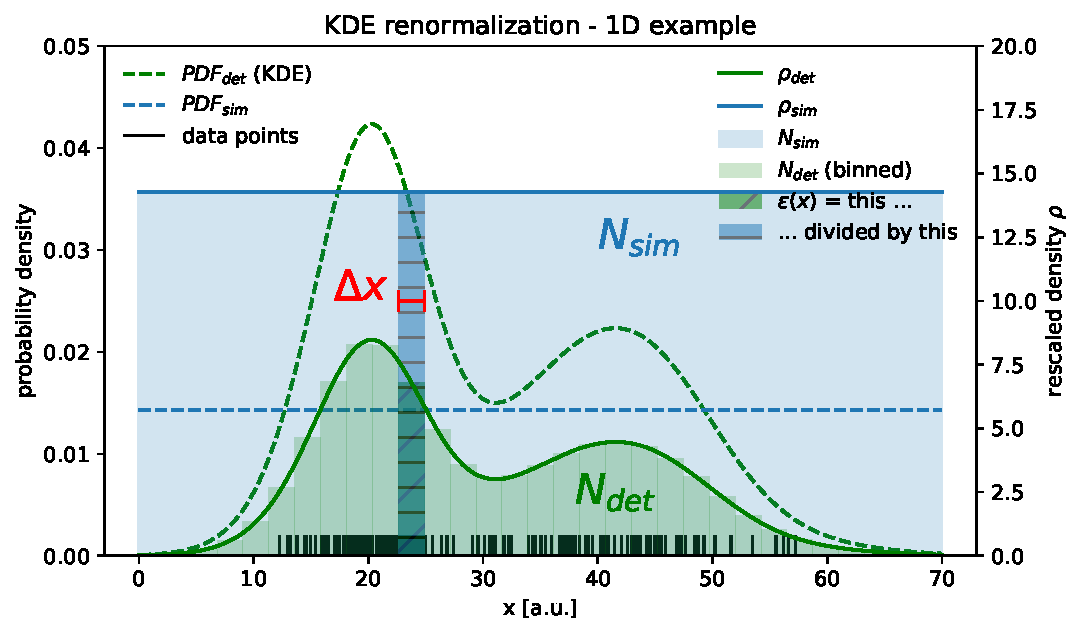
\includegraphics[width=\textwidth]{KDE_renorm_example.pdf}
	\caption[Example: KDE renormalization]{\textbf{Example: KDE renormalization.} 1D example to visualize the renormalization process. In this \enquote{toy simulation} \num{1000}~\enquote{photons} are simulated uniformly in the interval $[\SI{0}{\au},\SI{70}{\au}]$ for which the blue dashed line is the corresponding PDF. \num{200}~\enquote{photons} are detected (black dashes on the $x$-axis) and the PDF is calculated by adaptive kernel density estimation (green dashed line). Since the PDFs are both normalized to $1$ (w.r.t. left $y$-axis), a rescaling is now done (cf. right $y$-axis). The KDE for detected \enquote{photons} is scaled (green solid line) so that the enclosed area is $N_\text{det}=\num{200}$. This is also done with the PDF of simulated data (blue solid line) to correspond to an enclosed area $N_\text{sim}=\num{1000}$. The scaled detection and simulation densities $\rho_\text{det}$ and $\rho_\text{sim}$ are evaluated in bins with size $\Delta x$ which is analogous to the HEALPix area $\Omega_\text{HP}$ (cf. equation~\eqref{eq:omega_hp}). One gets the detection efficiency $\epsilon(x)$ for each bin by dividing the emphasized hatched areas by each other. The division of areas incorporates the integration over the HEALPix area done in the \enquote{real} evaluation (cf. equation~\eqref{eq:deteff}).}
	\label{deteff:1d_example}	
\end{figure}

\section{Application on Simulated Data}

The parameterization process introduced in section~\ref{sec:param:strategy} can now be applied to the simulation results from \geant. In the following sections, some comparisons and results are shown and discussed.

\subsection{Wavelength Binning}\label{sec:wvl_binning}

Since the photon detection efficiency of the SiPMs is a non-constant function of the wavelength (cf. figure~\ref{sipm:pde}), one can optimize the different wavelength ranges or \textit{bin sizes}~$\Delta\lambda$ by equalizing not the bin sizes (\textit{constant binning}) but the detected photons per bin which is further referred to as \textit{adaptive binning}. Figure~\ref{param:wvl_binning} shows a comparison between constant and adaptive wavelength binning.

\begin{figure}[H]
	\centering
	\begin{subfigure}[t]{0.49\textwidth}
		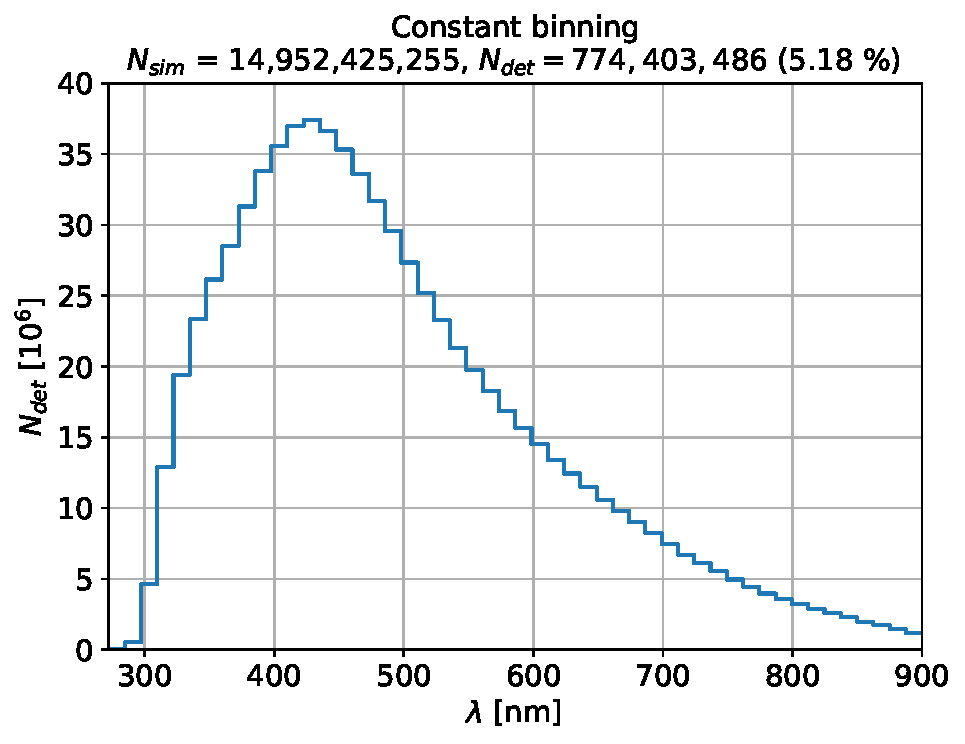
\includegraphics[width=\textwidth]{constant_wvl_bins_hist.pdf}
		\subcaption{constant binning}
		\label{param:wvl_binning:constant}
	\end{subfigure}
	\hfill
	\begin{subfigure}[t]{0.49\textwidth}
		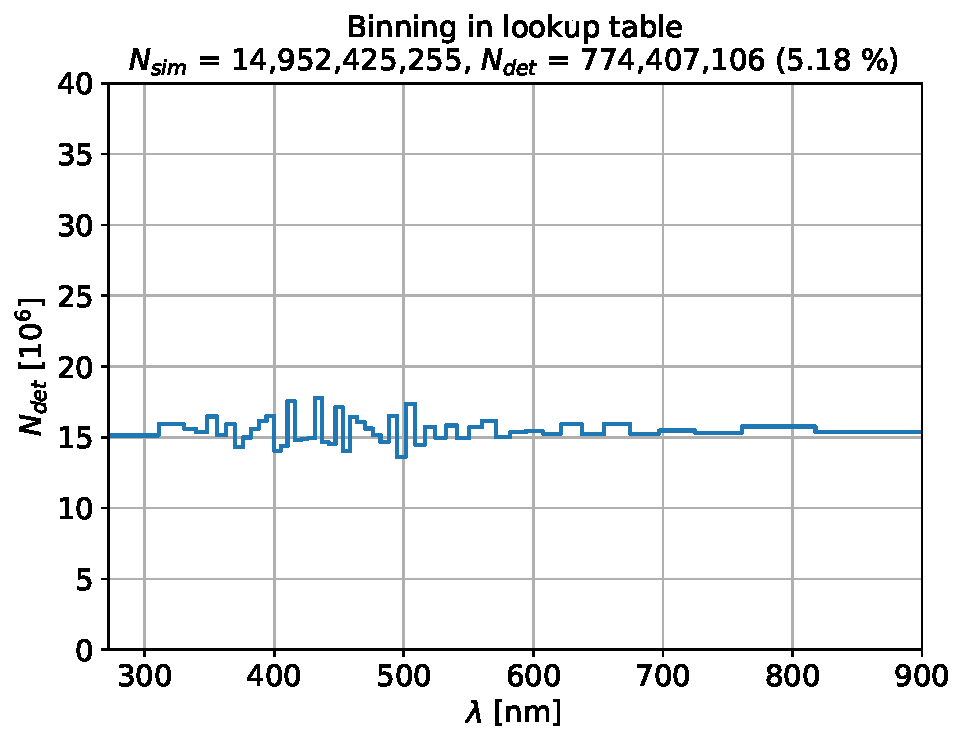
\includegraphics[width=\textwidth]{lut_wvl_bins_hist.pdf}
		\subcaption{adaptive binning}
		\label{param:wvl_binning:adaptive}
	\end{subfigure}
	\caption[Constant vs. adaptive wavelength binning]{\textbf{Constant vs. adaptive wavelength binning.} all wavelengths of photons that are detected by any camera SiPM are histogramized in \num{50} bins between \SI{272}{\nano\meter} and \SI{900}{\nano\meter}. In (\subref{param:wvl_binning:constant}), the \num{50} bins are distributed uniformly in wavelength so that one can see a shape that is quite similar to the PDE of the SiPMs. Figure~(\subref{param:wvl_binning:adaptive}) shows the same data with adaptive bin sizes to equalize the counts per bin. The resulting bin edges are rounded to integer numbers which causes the visible fluctuations.}
	\label{param:wvl_binning}
\end{figure}

The adaptive bin edges are calculated by sorting the wavelengths of all simulated particles that are detected by any of the 61 SiPM, i.e. all photons on which the KDE will be applied afterwards (cf. section~\ref{sec:adaptive_vs_nonadaptive}). Next, this sequence is divided into \num{50} parts of equal length. Thus, the wavelengths are divided into consecutive \SI{2}{\percent}-quantiles. In order to get more convenient bin sizes, the quantile limits (or bin edges) are rounded to integer values which obviously result in some fluctuations (cf. figure~\ref{param:wvl_binning:adaptive}).

With the adaptive wavelength binning it is ensured that in each range $\Delta\lambda$ almost the same number of photons is detected which enables a statistically more stable probability density estimation. The simulated wavelength range starts at $\lambda_\text{min}=\SI{272}{\nano\meter}$ since there is no photon detected with a wavelength below \SI{272}{\nano\meter} due to the absorption properties or the glass plate (cf. \ref{sec:iceact:model:material}).

\subsection{Adaptive vs. Non-adaptive KDE}\label{sec:adaptive_vs_nonadaptive}

Now that the wavelength binning is defined, the next step is to take a look on the camera pixels individually. Due to the distinct field of view of each pixel, the direction distribution of each pixel is characteristic and has regions with very different statistical densities as already stated in section~\ref{sec:adaptive_kde}. In order to get an idea of the given direction distributions for which the KDE should be calculated, figure \ref{param:example_scatter} shows some exemplary scatter plots of detected photons by an arbitrary camera pixel~$i$ in a wavelength range~$\Delta\lambda$.\\

\begin{figure}[H]
	\centering
	\begin{subfigure}[t]{0.49\textwidth}
		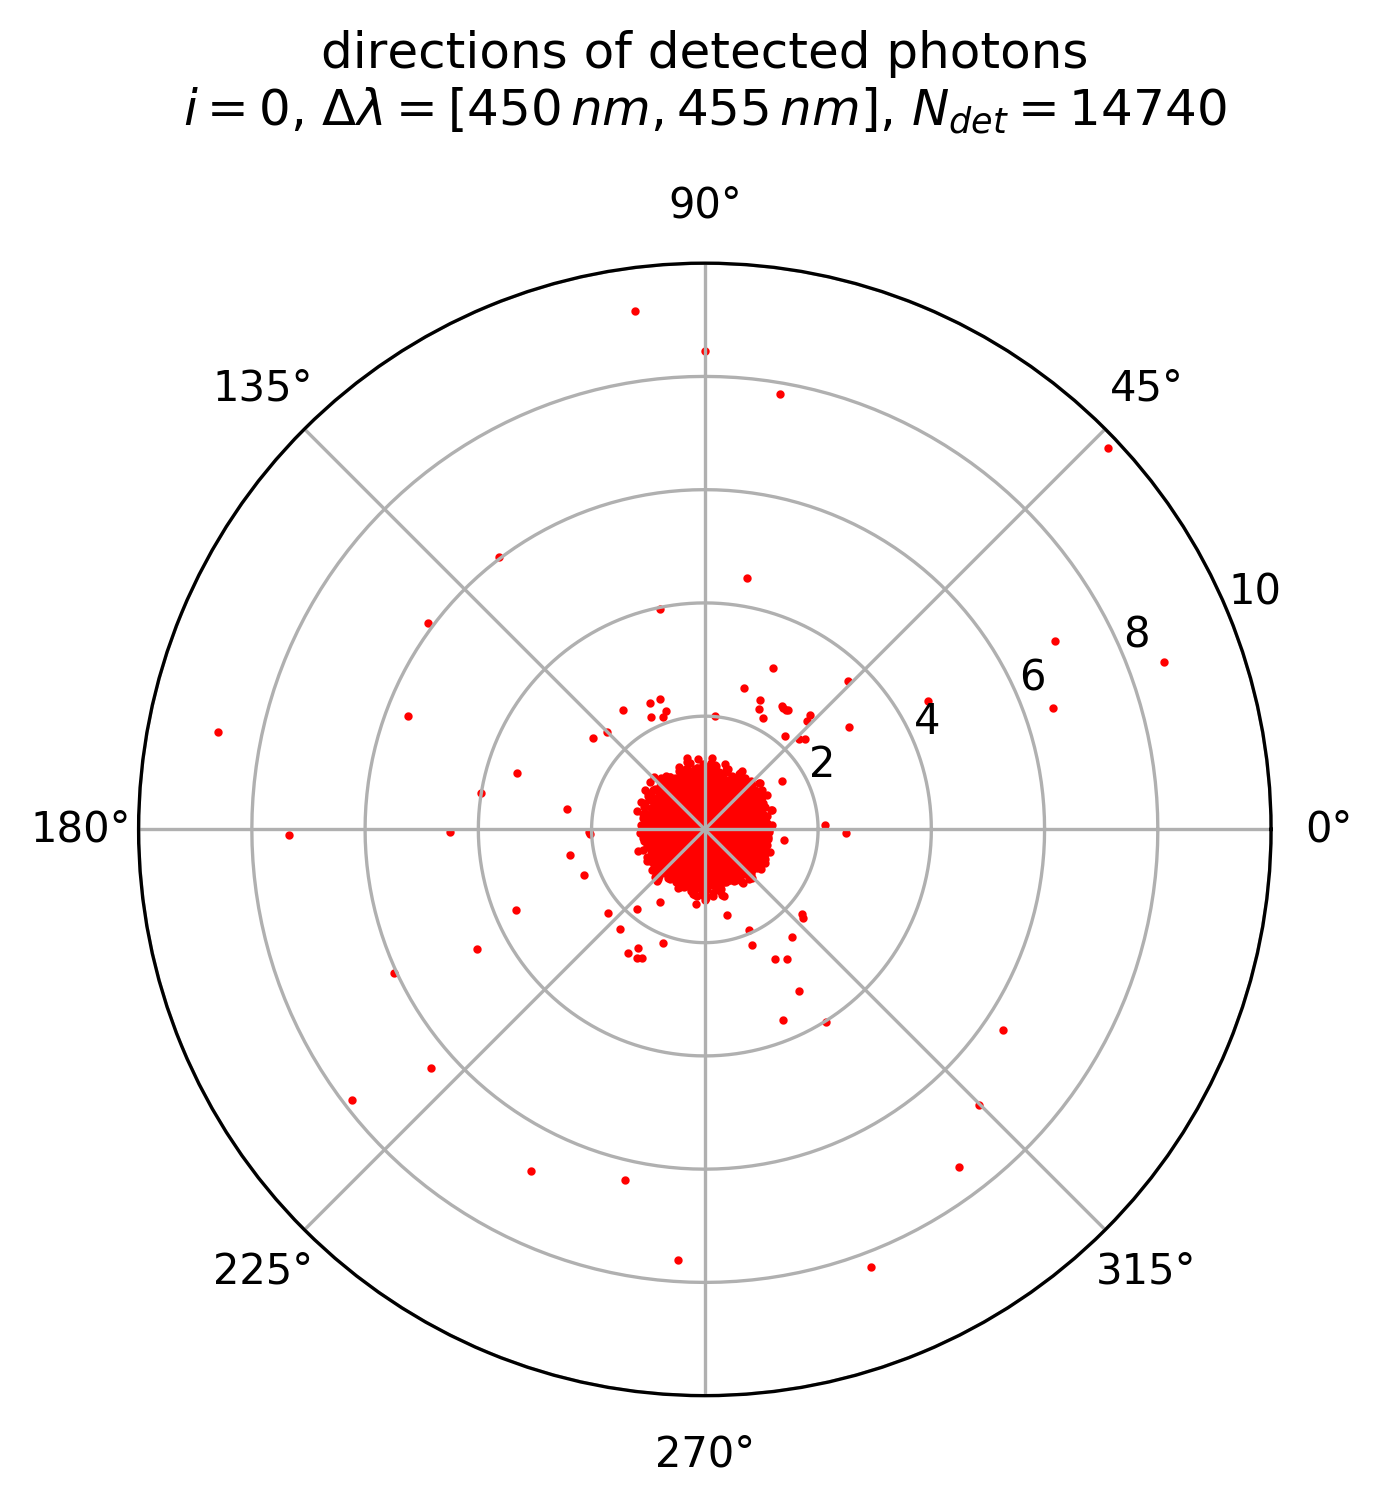
\includegraphics[width=\textwidth]{scatter_px00_wvl450-455nm.png}
		\subcaption{}
		\label{param:example_scatter:1}
	\end{subfigure}
	\hfill
	\begin{subfigure}[t]{0.49\textwidth}
		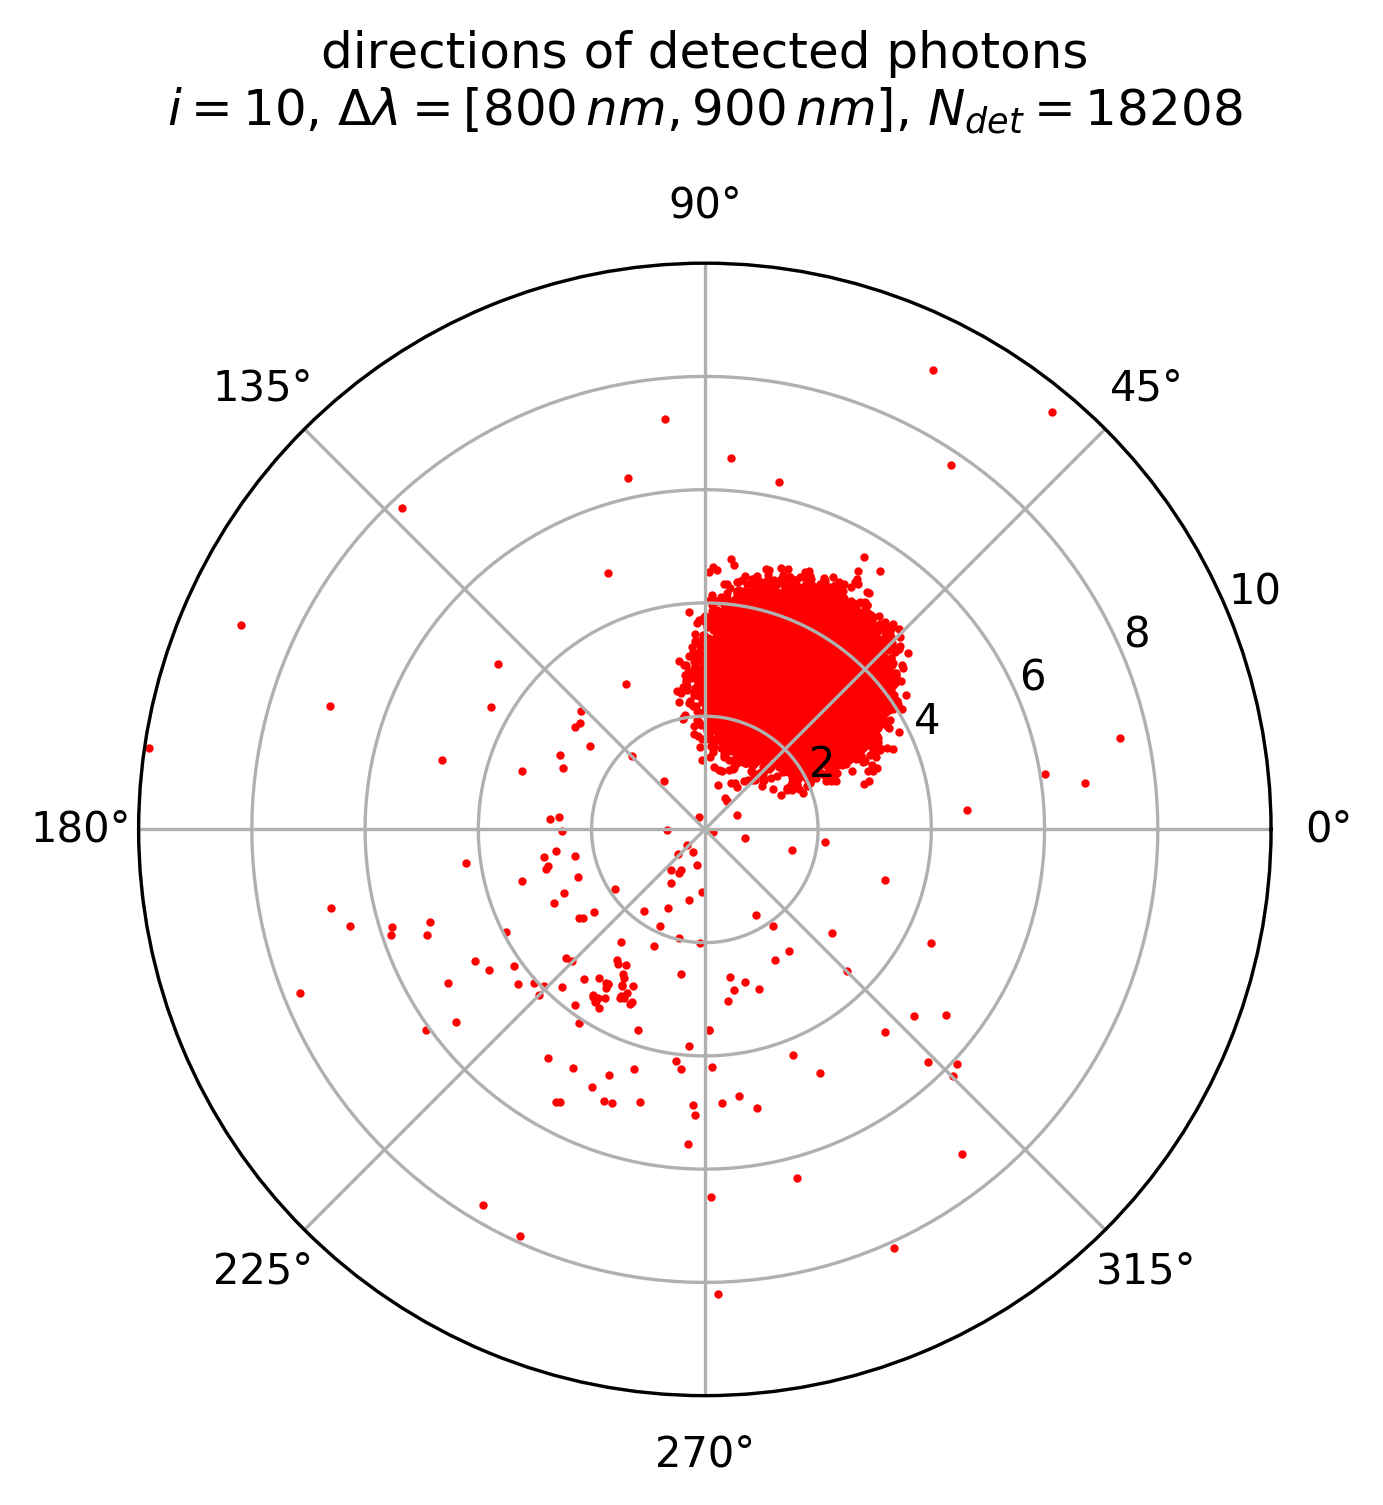
\includegraphics[width=\textwidth]{scatter_px10_wvl800-900nm.png}
		\subcaption{}
		\label{param:example_scatter:2}
	\end{subfigure}
	\vfill
	\begin{subfigure}[b]{0.49\textwidth}
		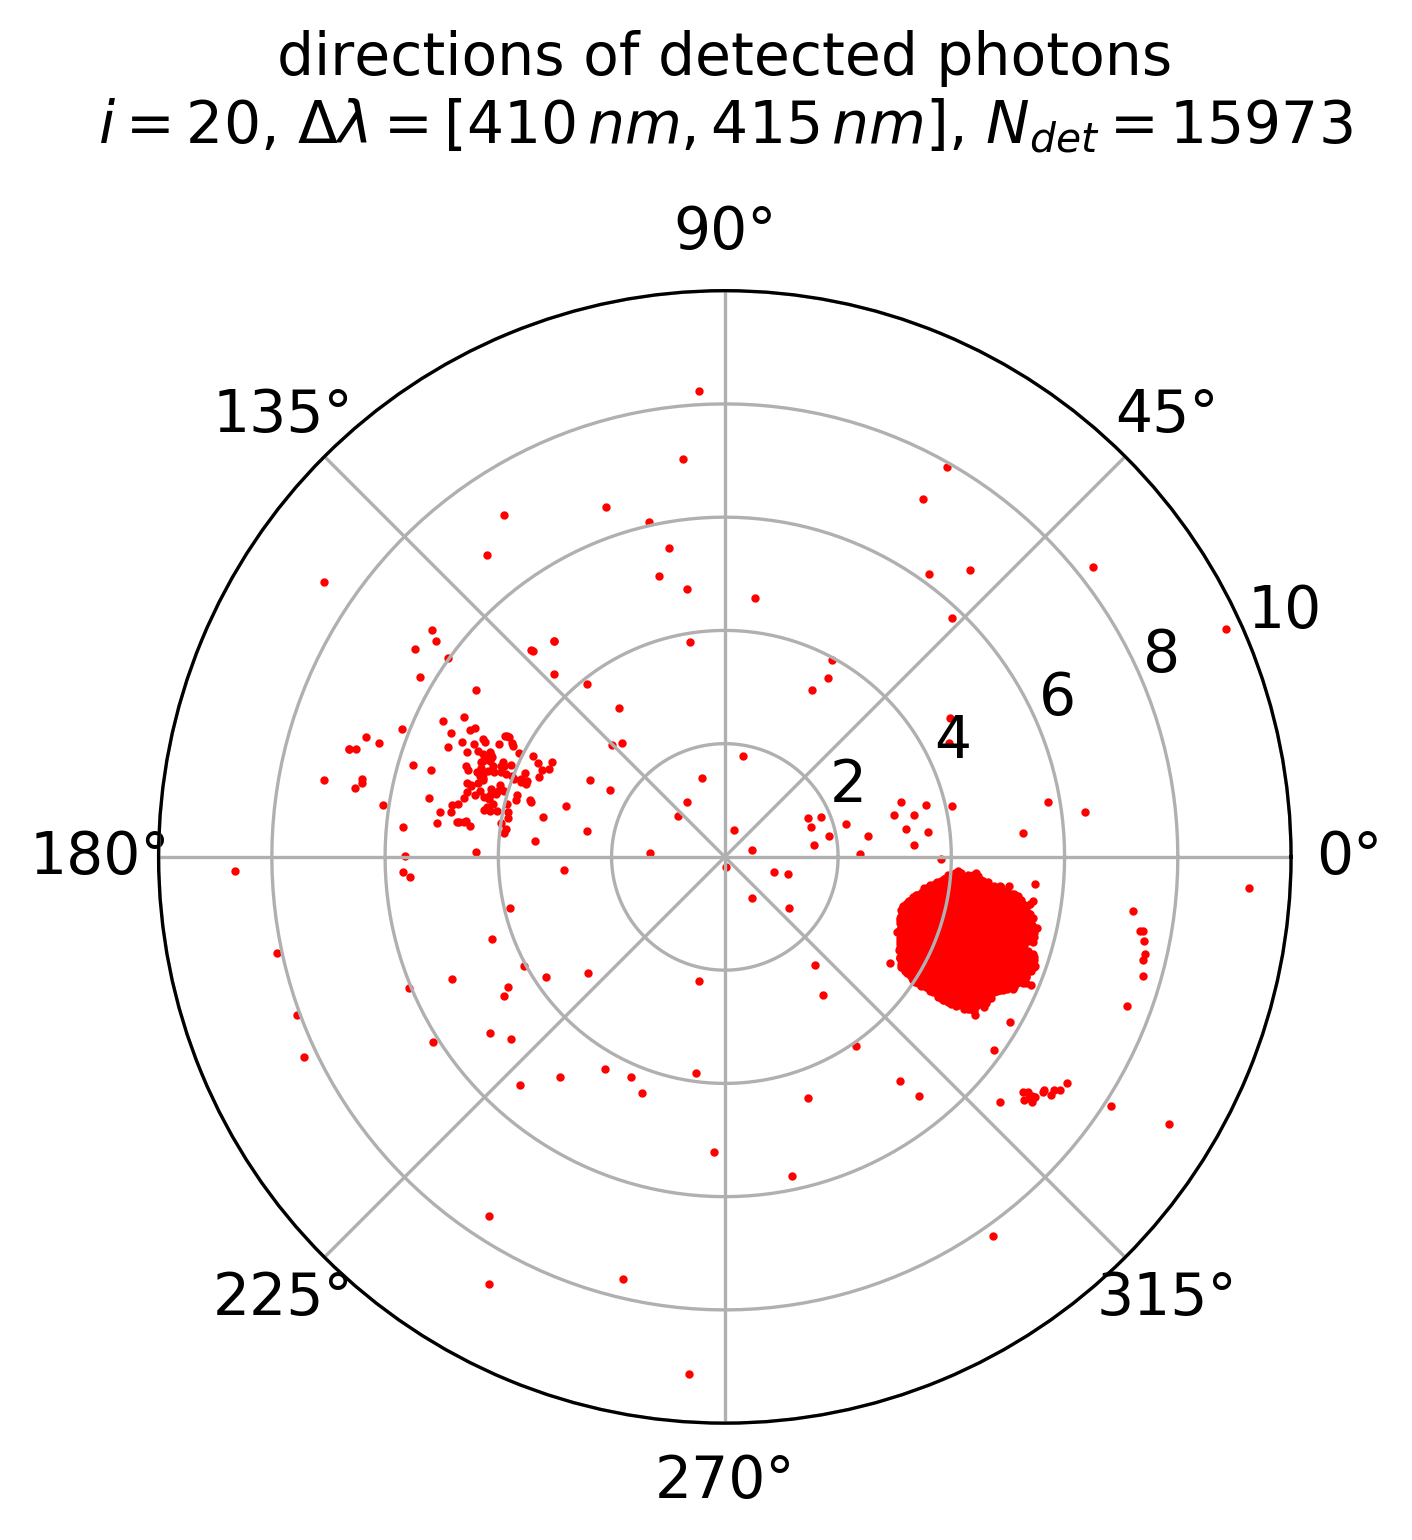
\includegraphics[width=\textwidth]{scatter_px20_wvl410-415nm.png}
		\subcaption{}
		\label{param:example_scatter:3}
	\end{subfigure}
	\hfill
	\begin{subfigure}[b]{0.49\textwidth}
		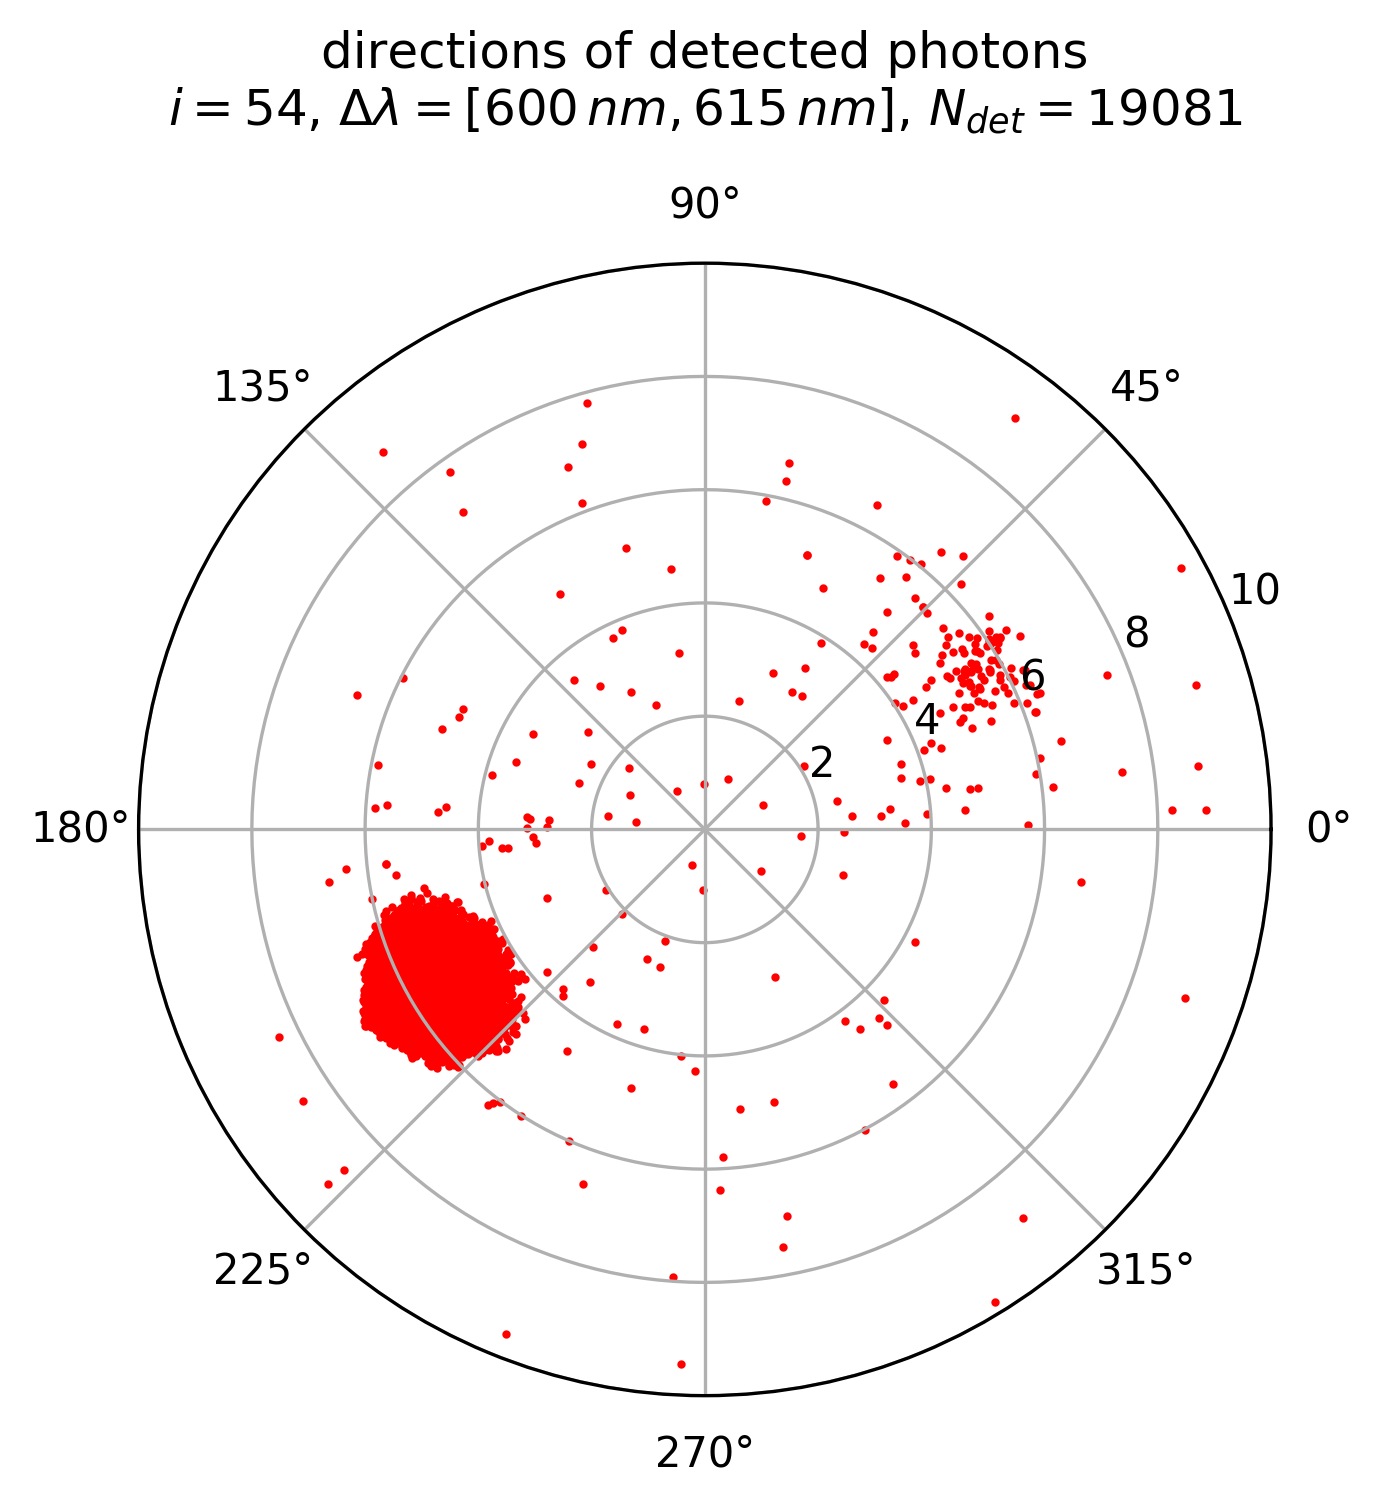
\includegraphics[width=\textwidth]{scatter_px54_wvl600-615nm.png}
		\subcaption{}
		\label{param:example_scatter:4}
	\end{subfigure}
	\caption[Example: directions of detected photons as a scatter plot]{\textbf{Example: directions of detected photons as a scatter plot.} A subset of simulated photon directions that are detected in a given camera pixel $i$ and the wavelength range $\Delta\lambda$ are shown in a polar plot. One can clearly see that there are regions with high and low statistical significance. Additionally, the \textit{ghost image} effect (cf. section~\ref{sec:ghost_image}) is visible in the non-central pixels ((\subref{param:example_scatter:2}), (\subref{param:example_scatter:3}), (\subref{param:example_scatter:4})).}
	\label{param:example_scatter}	
\end{figure}

The regions with very sparse \enquote{dots} can only arise from random scattering processes inside the optical system since they are outside the main field of view and the \textit{ghost image} region (cf. section~\ref{sec:ghost_image}). Thus, the probability density should be rather constant in these scattering regions. For the KDE, one achieves this by increasing the kernel bandwith. Simultaneously, the \enquote{real} detection regions should be described precisely which is done by reducing the bandwith. The need of an adaptive kernel density approach is given. Figure~\ref{param:kde_comparison} strikingly shows the difference between an adaptive and a non-adaptive KDE. Since the KDEs calculated there are only based on a small subsample of the simulation data, they may give the impression that the adaptive KDE still is very inaccurate in the scattering regions but on the full data sample this is not the case any more by having more scattered photons.\\

\begin{figure}[H]
	\centering
	\begin{subfigure}[t]{0.40\textwidth}
		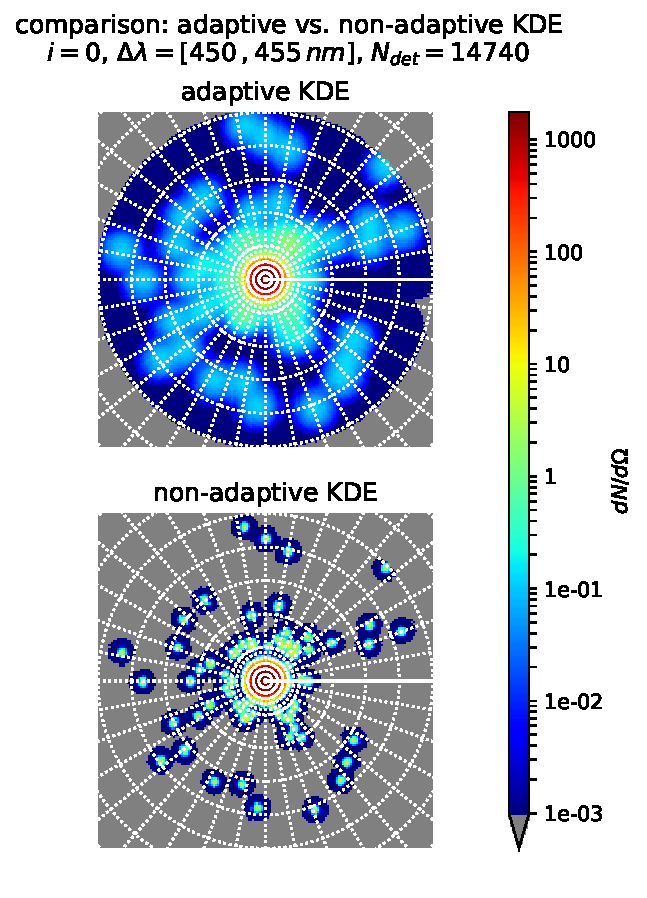
\includegraphics[width=\textwidth]{comparison_adaptive_nonadaptive_px00_wvl450-455.pdf}
		\subcaption{}
		\label{param:kde_comparison:1}
	\end{subfigure}
	\hfill
	\begin{subfigure}[t]{0.40\textwidth}
		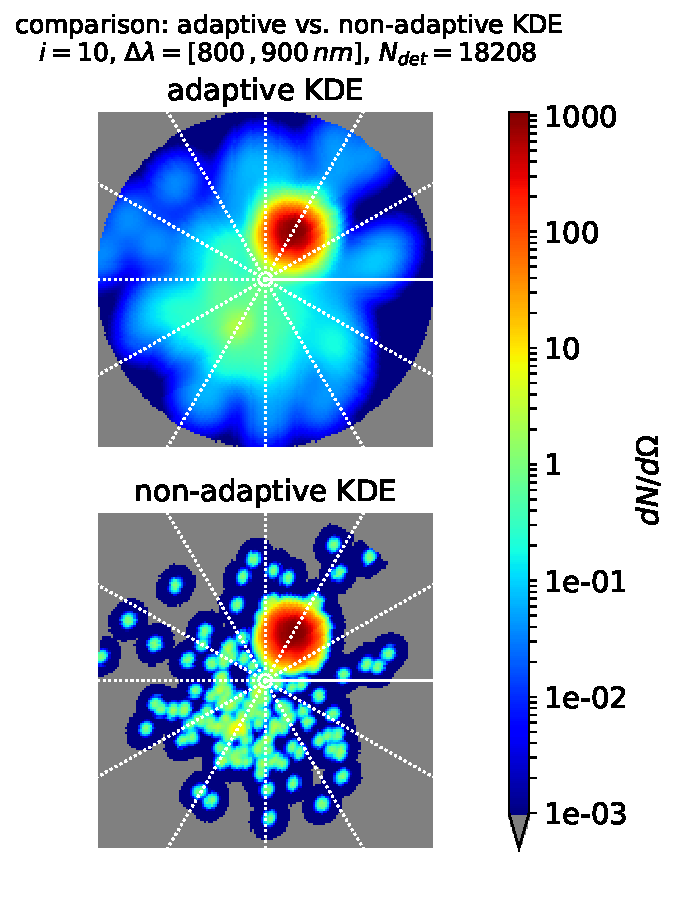
\includegraphics[width=\textwidth]{comparison_adaptive_nonadaptive_px10_wvl800-900.pdf}
		\subcaption{}
		\label{param:kde_comparison:2}
	\end{subfigure}
	\vfill
	\begin{subfigure}[b]{0.40\textwidth}
		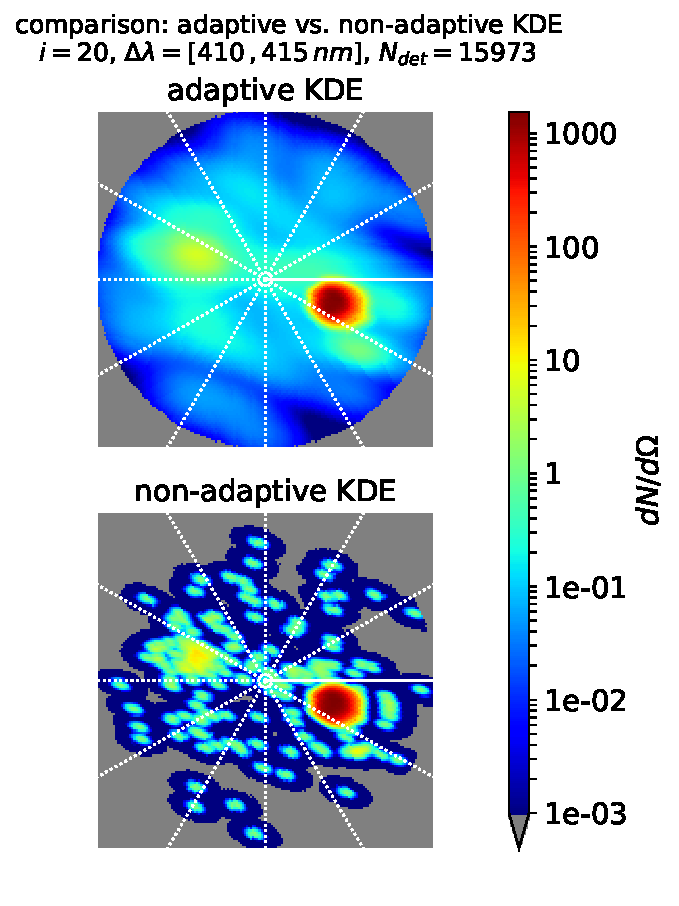
\includegraphics[width=\textwidth]{comparison_adaptive_nonadaptive_px20_wvl410-415.pdf}
		\subcaption{}
		\label{param:kde_comparison:3}
	\end{subfigure}
	\hfill
	\begin{subfigure}[b]{0.40\textwidth}
		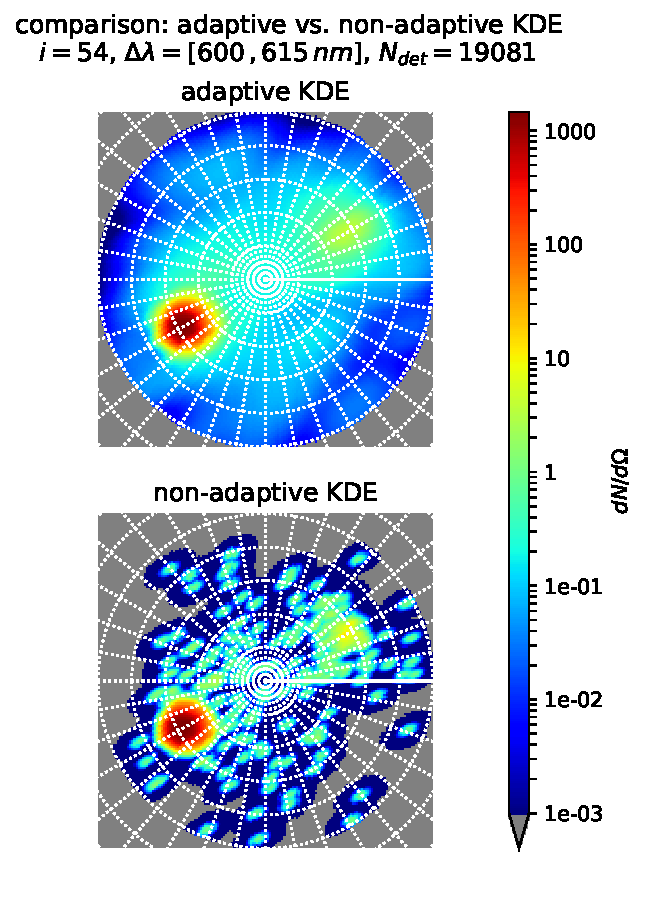
\includegraphics[width=\textwidth]{comparison_adaptive_nonadaptive_px54_wvl600-615.pdf}
		\subcaption{}
		\label{param:kde_comparison:4}
	\end{subfigure}
	\caption[Comparison: adaptive vs. non-adaptive KDE]{\textbf{Comparison: adaptive vs. non-adaptive KDE.} Evaluation of the direction distributions shown in figure~\ref{param:example_scatter} on a HEALPix grid with $N_\text{side}=\num{512}$. The plot shows a disc up to $\theta=\SI{10}{\degree}$ and the white dotted meridians have an azimuth distance of $\SI{30}{\degree}$. The azimuth $\phi$ starts at the solid white line and goes around counter-clockwise. Differences between an adaptive (top) and non-adaptive (bottom) KDE approach are visible. Especially in the region with low statistics (scattering region), the non-adaptive KDE is dominated by the fluctuations while adaptive KDE blurs the probability density more strongly.}
	\label{param:kde_comparison}		
\end{figure}

Anyway, the detection distributions can now be calculated and renormalized for each of the \num{61} camera pixels and \num{50} wavelength bins which result in \num{3050} so called \textit{detection efficiency maps} shown in the next section~\ref{sec:deteff_maps}.

\subsection{Detection Efficiency Maps}\label{sec:deteff_maps}

By follow the strategy described in section~\ref{sec:param:strategy} and considering the findings from sections~\ref{sec:wvl_binning} and \ref{sec:adaptive_vs_nonadaptive}, one can now finally calculate \textit{detection efficiency maps}. For each camera pixel $i$ and wavelength bin $\Delta\lambda$, these maps show the probability $\epsilon_{i,\Delta\lambda,HP}$ to detect a photon with wavelength $\lambda\in\Delta\lambda$ in camera pixel $i$ as a function of its origin direction~$(\theta,\phi)$ which is coded in the ordinal number~$HP$ of the corresponding HEALPix. For the pixelization parameter of the HEALPix model~$N_\text{side}$, one has to choose a reasonable value (cf. table~\ref{healpix:table}): too fine pixelization would obviously result in a very detailed parameterization. Due to KDE, an \enquote{unbinned} detection efficiency is available -- at least in origin directions -- so that it is technically possible to choose a very fine binning. The problem is, that the main goal of the \iceact parameterization is to produce a lookup table that is efficient and capable of evaluating large amounts of Cherenkov photons. A unnecessarily fine HEALPix binning would just blow up the lookup table and quick evaluation is not feasible any more.

\todo{central pixel, FOV einzeichnen, vernünftige wahl von Nside zeigen}

\todo{maps von neuer rechnung, die hoffentlich noch fertig wird}

\todo{absolut höchste Effizienz erwähnen ... welche Richtung, welcher pixel, welche wellenlänge}

\section{Lookup Table (LUT)}

As the detection efficiency maps are ready now, one has to think about a way to access the information as fast as possible. Usually, this is done by storing the parameterization function evaluated at certain points in a multidimensional array structure known as \textit{lookup table}. Afterwards, events can be \enquote{diced} with the given information yielding count histograms for the camera -- named \textit{images}.

\subsection{LUT Production}\label{sec:lut_production}

First of all, one has to define how to iterate over the given information. In this case, one starts with a photon direction $(\theta,\phi)$ translated into the corresponding HEALPix number~$HP$ and the wavelength~$\lambda$ of this photon which is assigned to the proper wavelength bin~$\Delta\lambda$. The result then should be the response of each pixel to the very same photon, i.e. how probable is it for the photon to be detected in camera pixel $i$. In order to achieve this, one can evaluate the detection efficiency maps by fist considering just one HEALPix. For this HEALPix, the detection efficiency for all wavelength bins and all camera pixels is read out, which is shown exemplary in figure~\ref{lut:transpose_example}. 

\begin{figure}[H]
	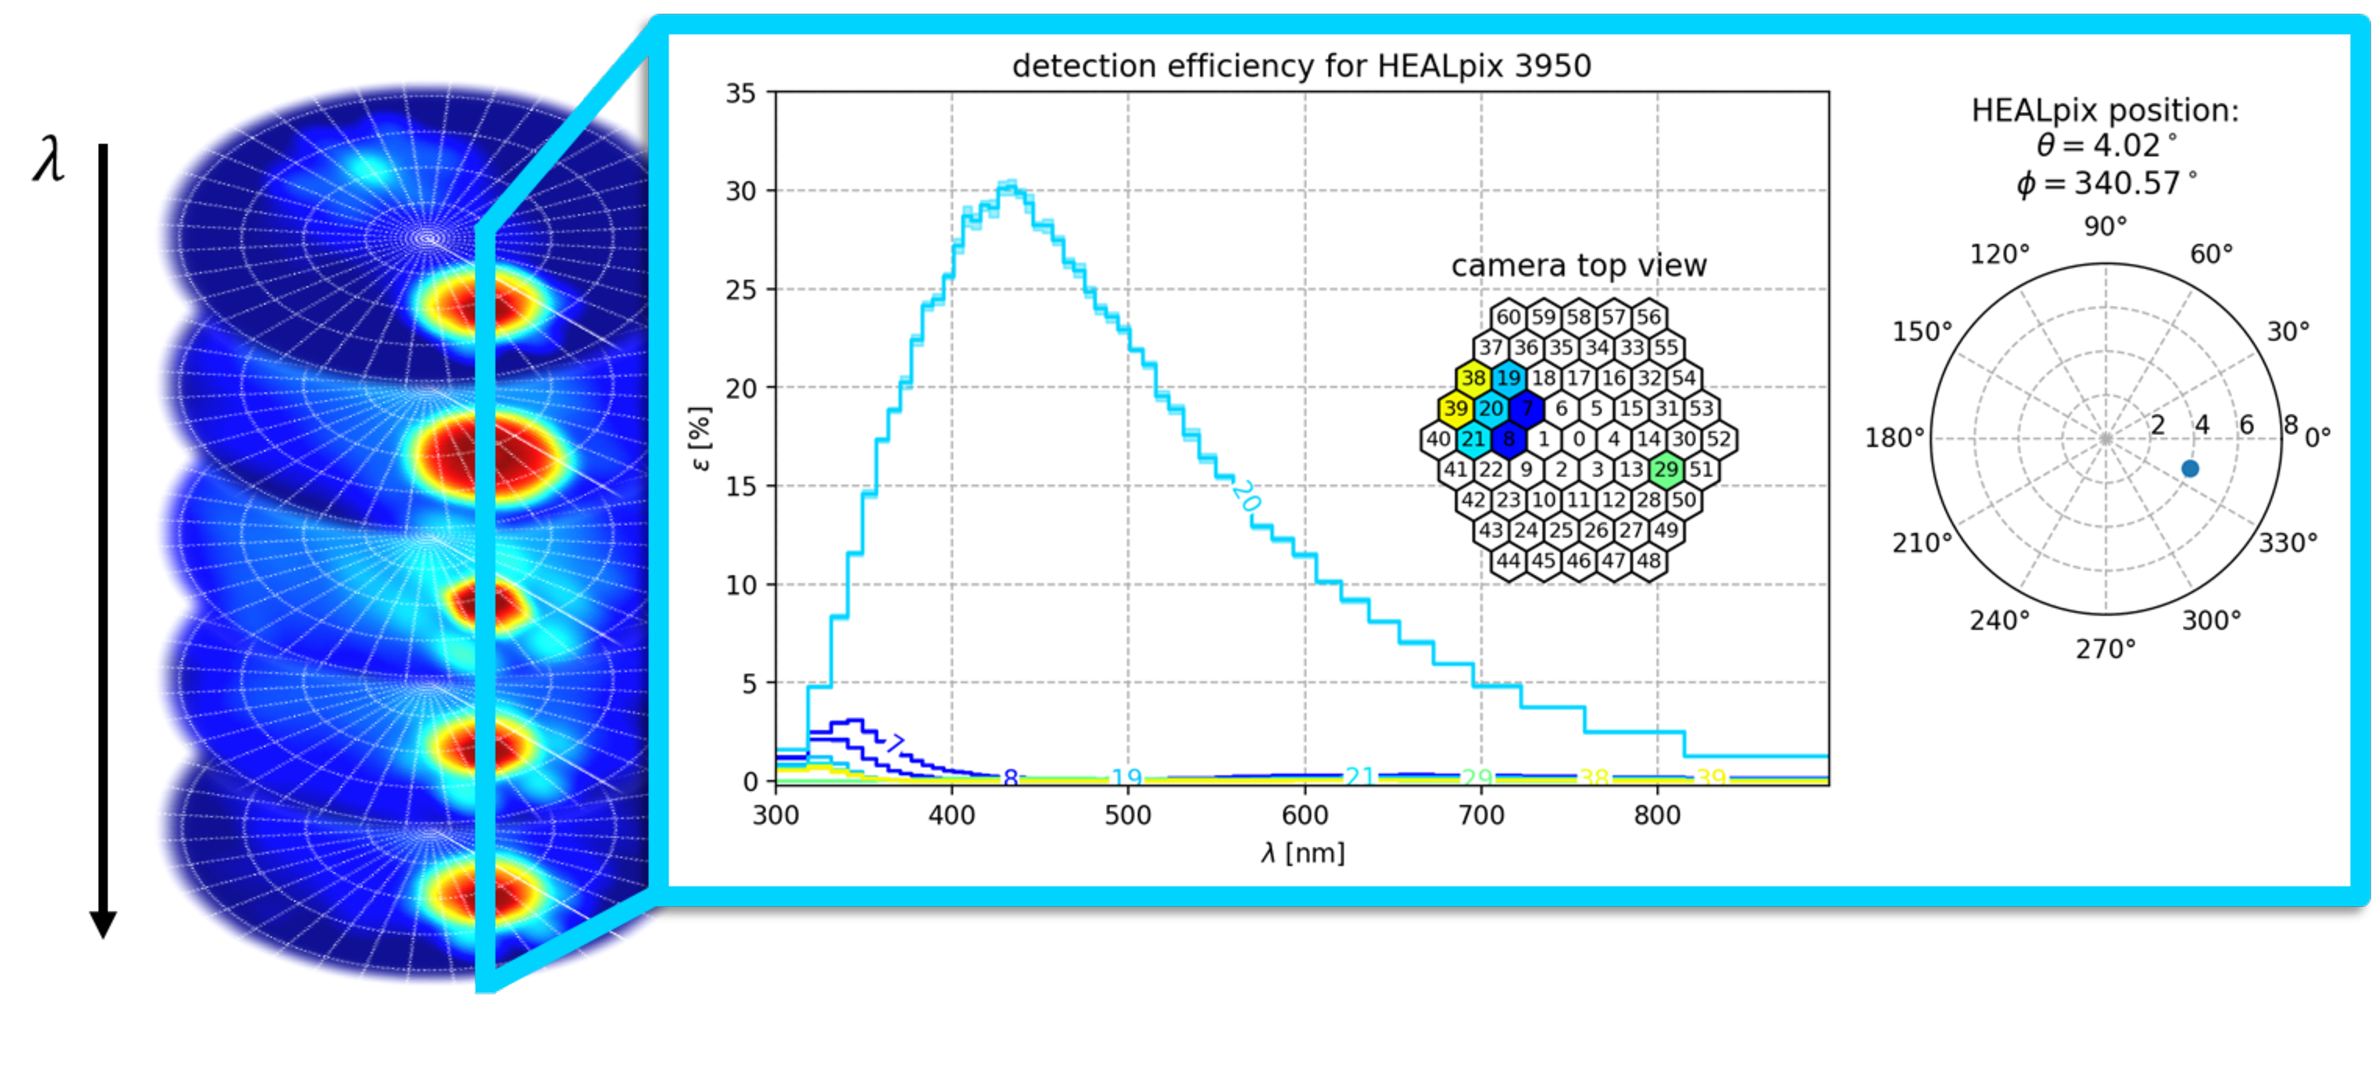
\includegraphics[width=\textwidth]{LUT_transposition_example.pdf}
	\caption[Visualization for the lookup table transposition]{\textbf{Visualization for the lookup table transposition.} A certain HEALPix (here: $HP=\num{3950}$) is considered. For one camera pixel, the detection efficiency is read from the maps throughout all wavelength bins. In this example, some maps for pixel \num{20} are chosen. Doing this for all camera pixels yields to the blue-framed plot. For the considered HEALPix one gets the wavelength-dependent detection efficiency for each camera pixel. The \enquote{camera top view} plot shows the camera as seen from the lens. Pixels that have a maximum detection efficiency greater than~\SI{0.1}{\percent} are emphasized with colors. The detection efficiency functions of all other pixels are not plotted. Besides, the HEALPix center coordinates are given with a polar plot.}
	\label{lut:transpose_example}
\end{figure}

By iterating over each HEALPix of one gets $N_{HP}\times N_{\Delta\lambda}$ pixel-by-pixel detection efficiency arrays where $N_{HP}$ is the total number of HEALPix covered by simulation and $N_{\Delta\lambda}$ the number of wavelength bins. These sub-arrays are further named as $\epsilon_{HP,\Delta\lambda}$ and contain the detection efficiency $\epsilon_i$ for each camera pixel $i$ (also called \textit{pixel response}). 

Additionally, one can even improve the structure of these sub-array by not just saving the single responses $\epsilon_i$ ordered by pixel number, but saving the cumulative responses. Then, the $k$-th of totally \num{60} elements in the sub-array is defined as 
\begin{align}
	\epsilon^\text{abs}_k = \sum_{i=0}^{k} \epsilon_i\,,
	\label{eq:eps_cumulative}
\end{align}
i.e. $\epsilon^\text{abs}_k$ is the probability to detect the photon in any pixel with number $i\in[0,k]$. Additionally, it is
\begin{align}
\epsilon_k^\text{abs} < 1\,,
\end{align}
where the last element $\epsilon_{60}^\text{abs}$ is the total detection probability of the camera and distances between the elements represent the responses of the individual camera pixels. The advantage of saving the cumulative sum rather than actual responses gets clear in the next section~\ref{sec:lut_readout}. Schematically, the lookup process can be described by
\begin{align}
	\gamma \rightarrow
	\begin{cases}
		(\theta,\phi) & \rightarrow HP\\
		\lambda & \rightarrow \Delta\lambda
	\end{cases}
	\Rightarrow \epsilon^\text{abs}_{HP,\Delta\lambda} = \{\epsilon^\text{abs}_k\}_{k=0}^{60}\,.
\end{align}\\

The HEALPix resolution used for parameterization of \iceact is $N_\text{side}=\num{512}$. With $\theta_\text{max}=\SI{10}{\degree}$, this results in a total \enquote{active} HEALPix number of $N_{HP}=\num{24420}$. Additionally, the wavelengths are divided into $N_{\Delta\lambda} = \num{50}$ bins in the interval $[\SI{272}{\nano\meter},\SI{900}{\nano\meter}]$ (cf. section~\ref{sec:wvl_binning}). For the \num{61} pixel camera this results in $N_{HP}\cdot N_{\Delta\lambda}\cdot \num{61} = \num{74481000}$ numbers to be saved. The needed disk space for this lookup table is \SI{284}{\mebi\byte} by using \SI{32}{\bit} float as data type\footnote{Since also the information about wavelength binning, HEALPix model, and maximum simulated zenith angle has to be included, the lookup table file might need slightly more space}.

\subsection{LUT Readout -- \enquote{Event Dicing}}\label{sec:lut_readout}

Now that the data is ready, an evaluation algorithm has to be elaborated. In the following, the principle to evaluate $N$ photons is described step by step.

\begin{enumerate}
	\item For each direction the corresponding HEALPix number is calculated.\footnote{In this thesis, the evaluation algorithm is implemented with Python. For HEALPix calculations, the package \textit{healpy} is used.}
	\begin{align}
		\{(\theta_i, \phi_i)\}_{i=1}^N \rightarrow \{HP_i\}_{i=1}^N
	\end{align}
	\item Only valid photons are evaluated. A photon is valid if its HEALPix number~$HP_i$ is in the lookup table -- i.e. below the cutoff -- and if its wavelength~$\lambda_i$ is in the wavelength range covered by the lookup table $[\lambda_\text{min},\lambda_\text{max}]$. $N^\ast\leq N$ photons are valid. Invalid photons are counted.
	\begin{align}
		\text{valid} \coloneqq HP_i < N_{HP} \wedge \lambda_i \in [\lambda_\text{min},\lambda_\text{max}]
	\end{align} 
	\item For all $N^\ast$ photons, the corresponding wavelength bin is determined.
	\begin{align}
		\{\lambda_{i^\ast}\}_{i^\ast=1}^{N^\ast} \rightarrow \{ \Delta\lambda_{i^\ast} \}_{i^\ast=1}^{N^\ast}
	\end{align}
	Here, the index of the assigned wavelength bin rather than the actual range is important for the lookup table query.
	\item The actual lookup table query is performed. Thus, every valid photon gets its proper pixel response array.
	\begin{align}
		\{HP_{i^\ast}, \Delta\lambda_{i^\ast}\}_{i^\ast=1}^{N^\ast} \rightarrow \{ \epsilon^\text{abs}_{HP_{i^\ast},\Delta\lambda_{i^\ast}}\}_{i^\ast=1}^{N^\ast}
	\end{align}
	\item For each valid photon $i^\ast$, a random number $r_{i^\ast}\in[0,1)$ is diced and sorted into the corresponding response array. Now, the advantage of saving the cumulative rather than the absolute responses (cf. section~\ref{sec:lut_production}) becomes clear. By definition, the cumulative responses are sorted in ascending order\footnote{This is the case if all numbers are non-negative like it is the case for the camera pixel responses. Otherwise, the cumulative sequence may not be sorted.}. As a result, the position $k$ where the random number is sorted in equals the number of the camera pixel where the photon is detected. If the random number is sorted in at the \num{61}-th position -- i.e. at the end -- this means that the photon is not detected. The cumulative saving enables a lookup process that is only based on comparative operations which are very fast.
	\item The resulting sorting positions $k_{i^\ast}$ can now be histogramized which gives the final image seen by the camera.
\end{enumerate}

\section{Application on CORSIKA Air Showers Events}


% -----------------------------------
\backmatter
	\renewcommand{\listfigurename}{Figures}
	\listoffigures 				% Abbildungsverzeichnis
	\protect\thispagestyle{scrheadings}
	\renewcommand{\listtablename}{Tables}
	\listoftables				% Tabellenverzeichnis
	\protect\thispagestyle{scrheadings}
	\pagestyle{scrheadings}
	\printbibliography[title=Literature]

\end{document}